\begin{figure}[htbp]
\centering
\begin{tabular}{ccc}
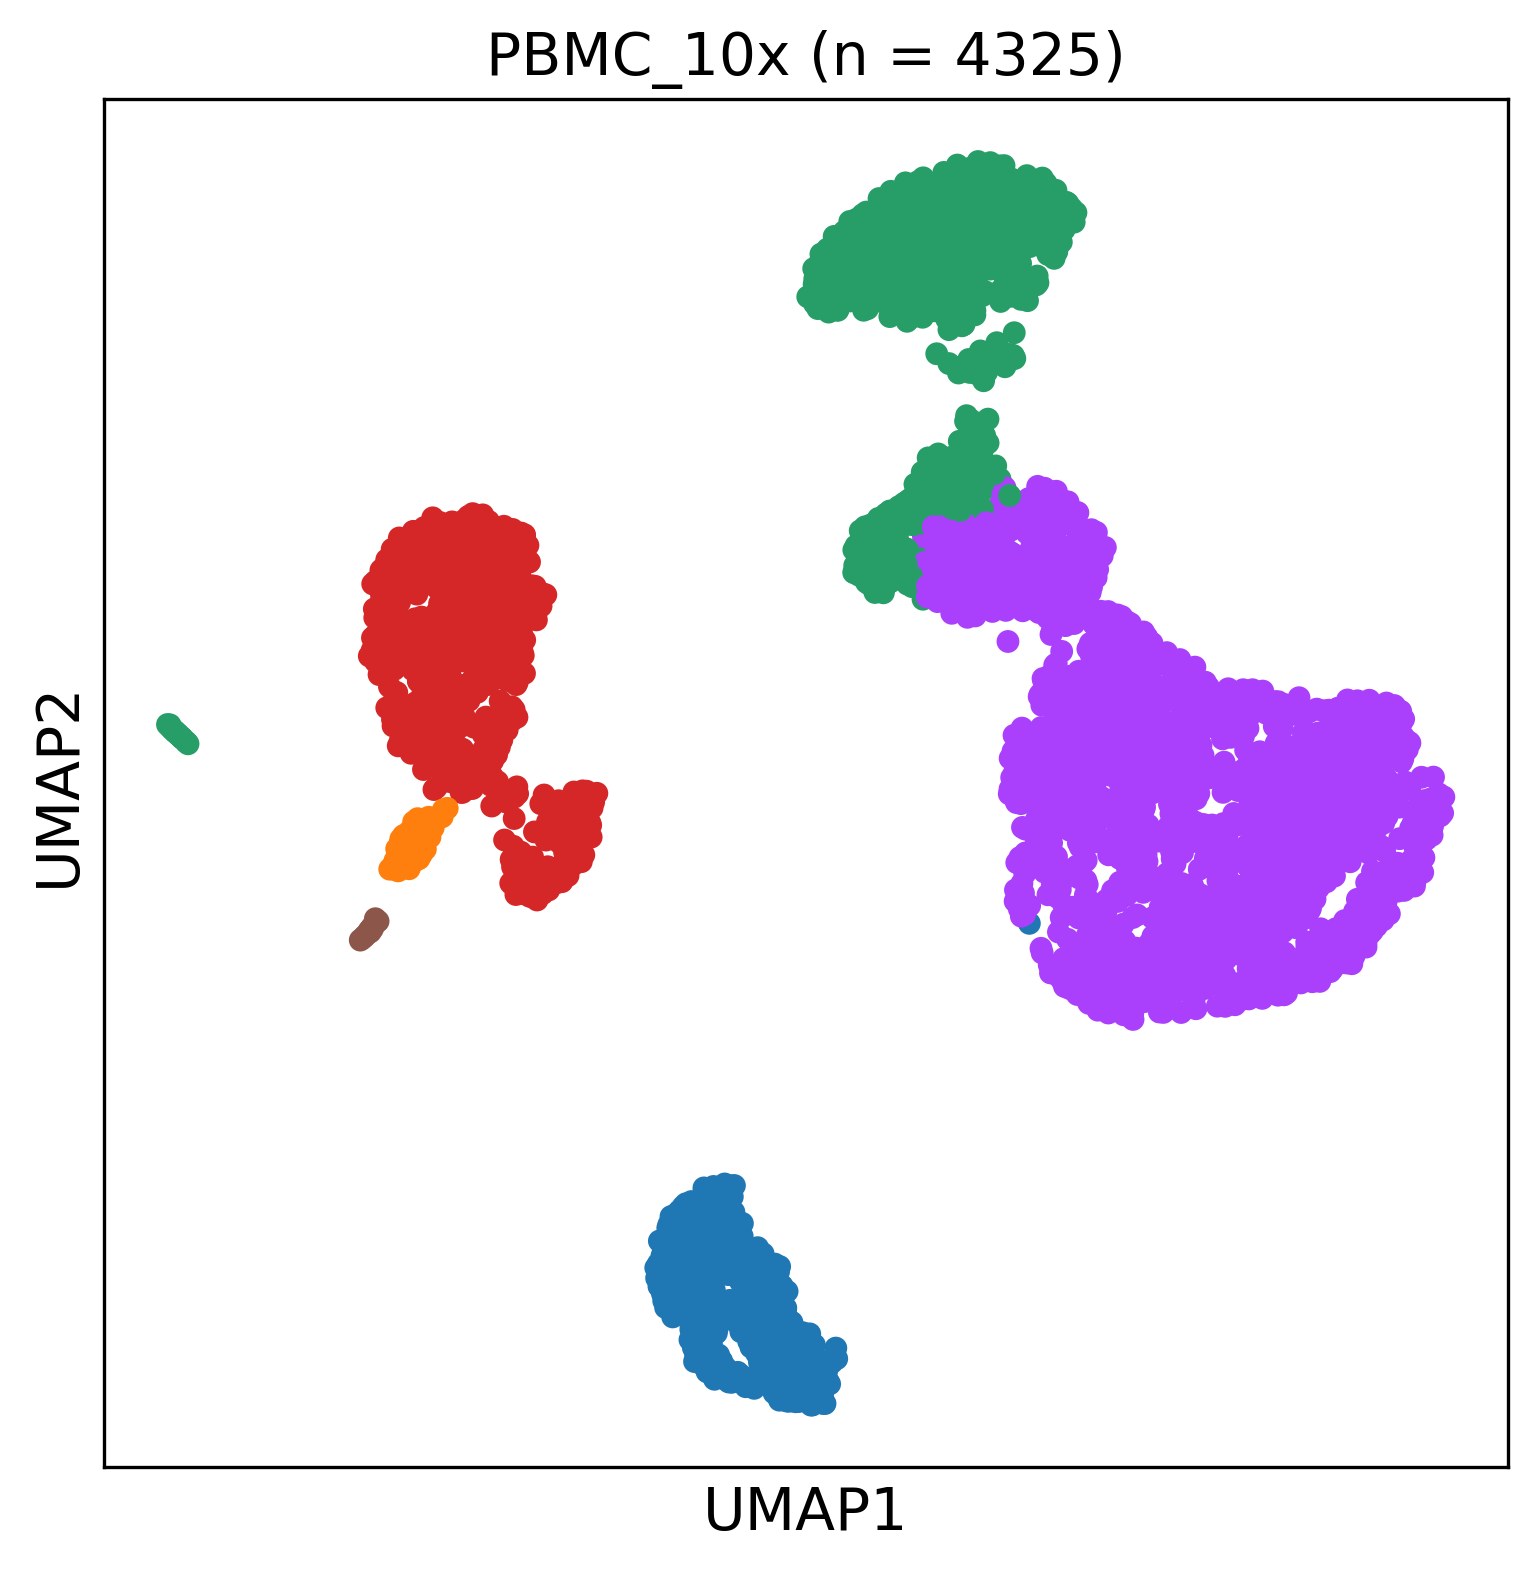
\includegraphics[width=0.25\textwidth]{images/clusterings/PBMC_10x.png} &
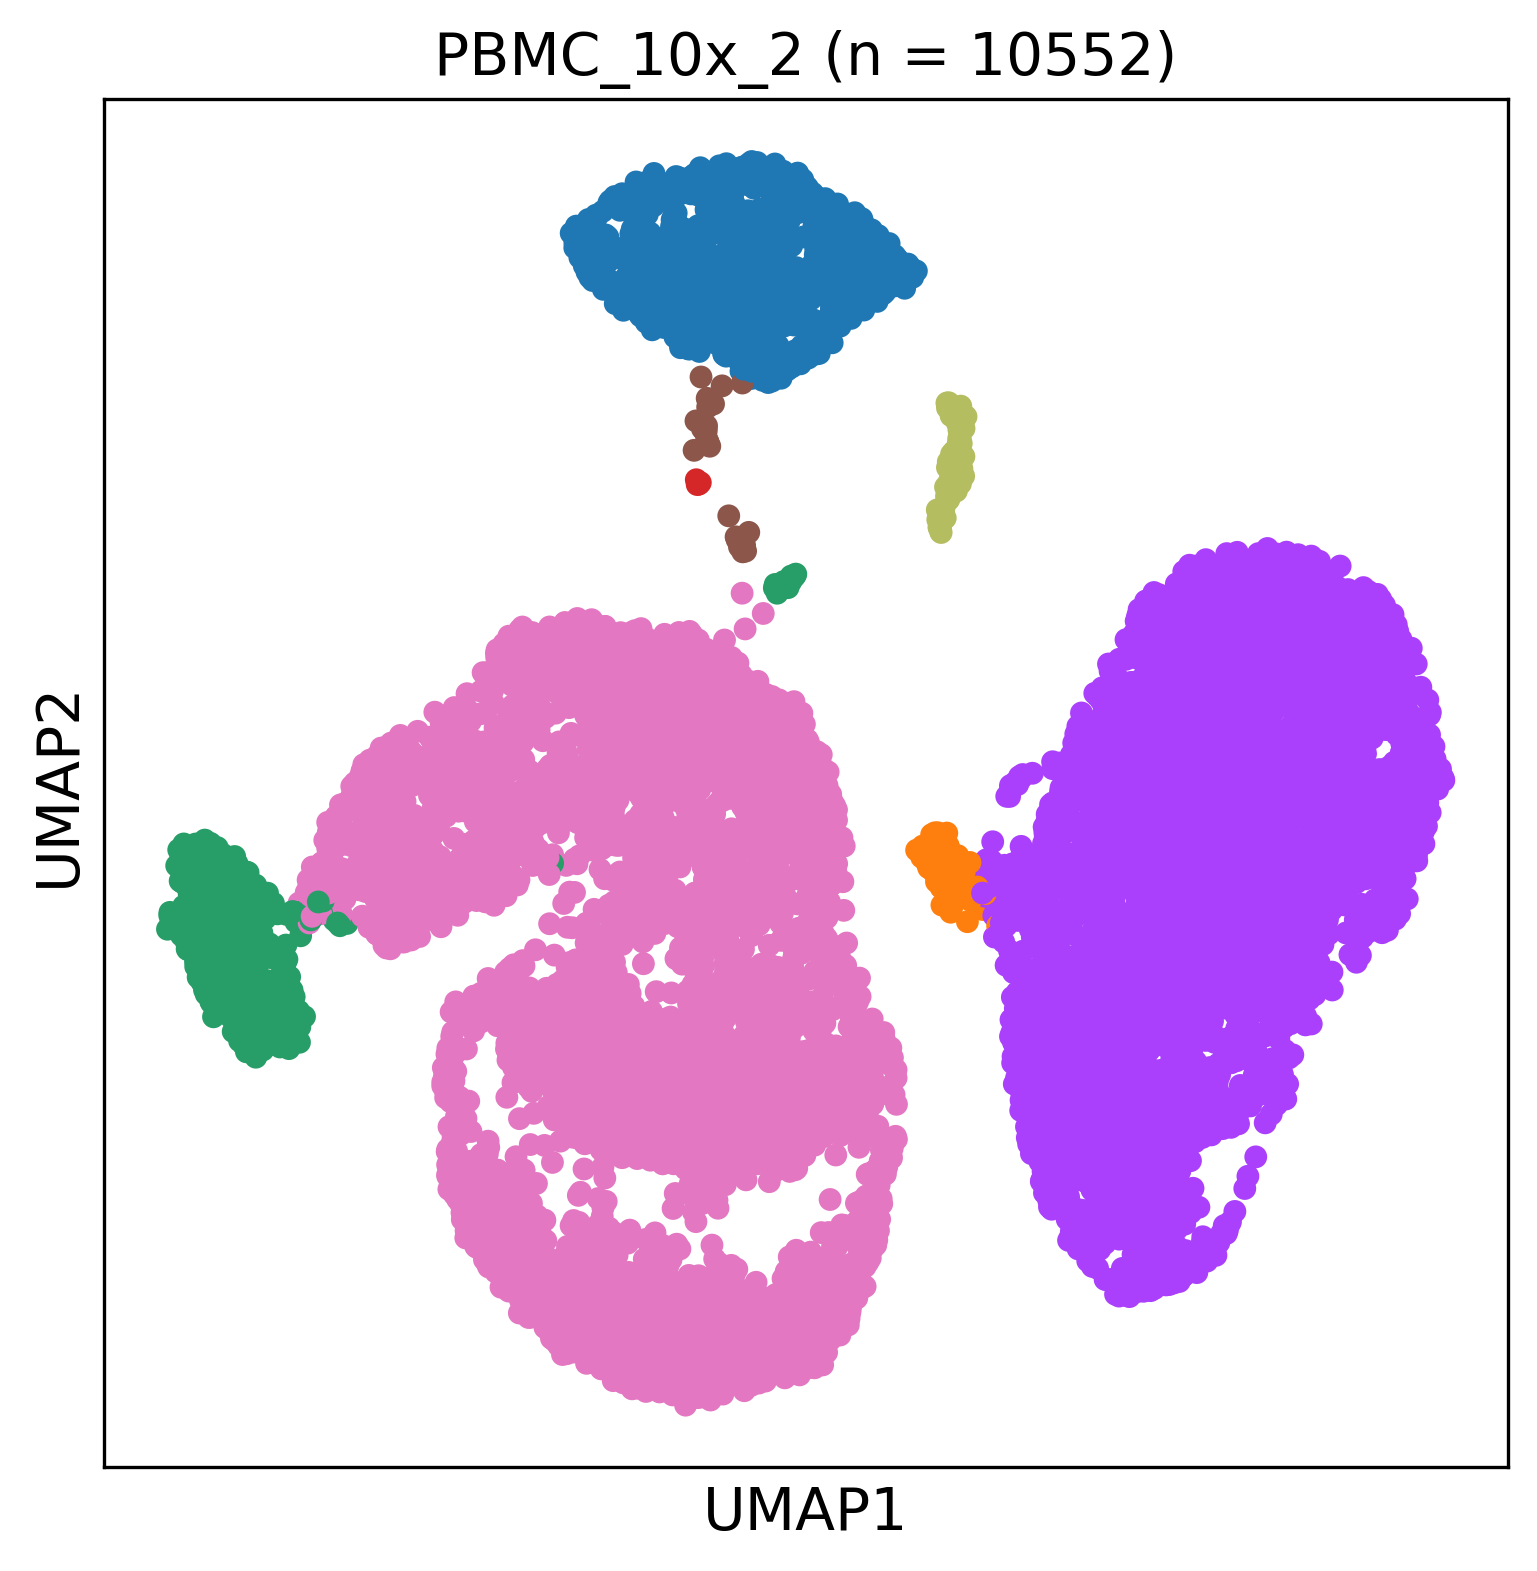
\includegraphics[width=0.25\textwidth]{images/clusterings/PBMC_10x_2.png} &
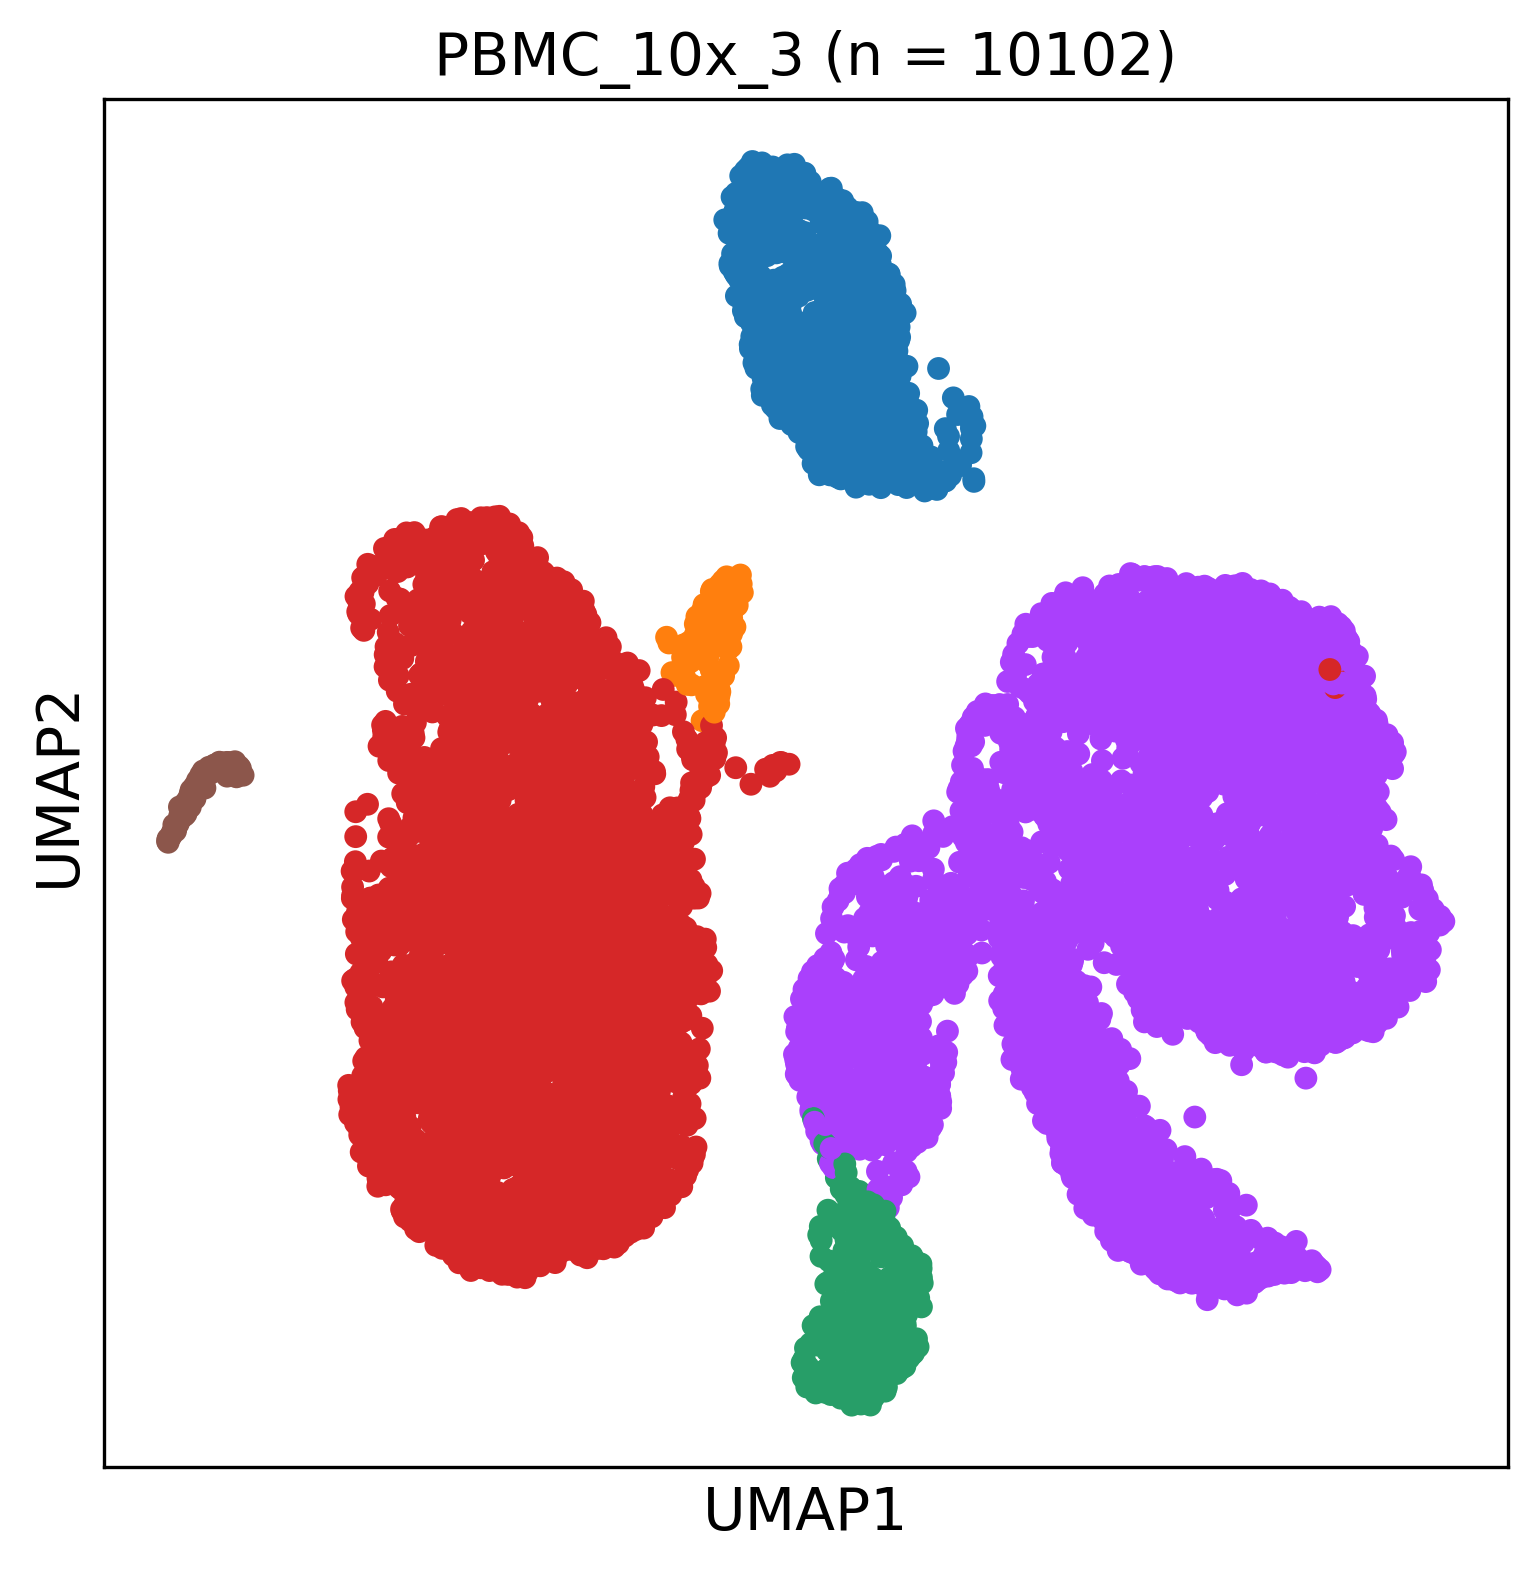
\includegraphics[width=0.25\textwidth]{images/clusterings/PBMC_10x_3.png} \\
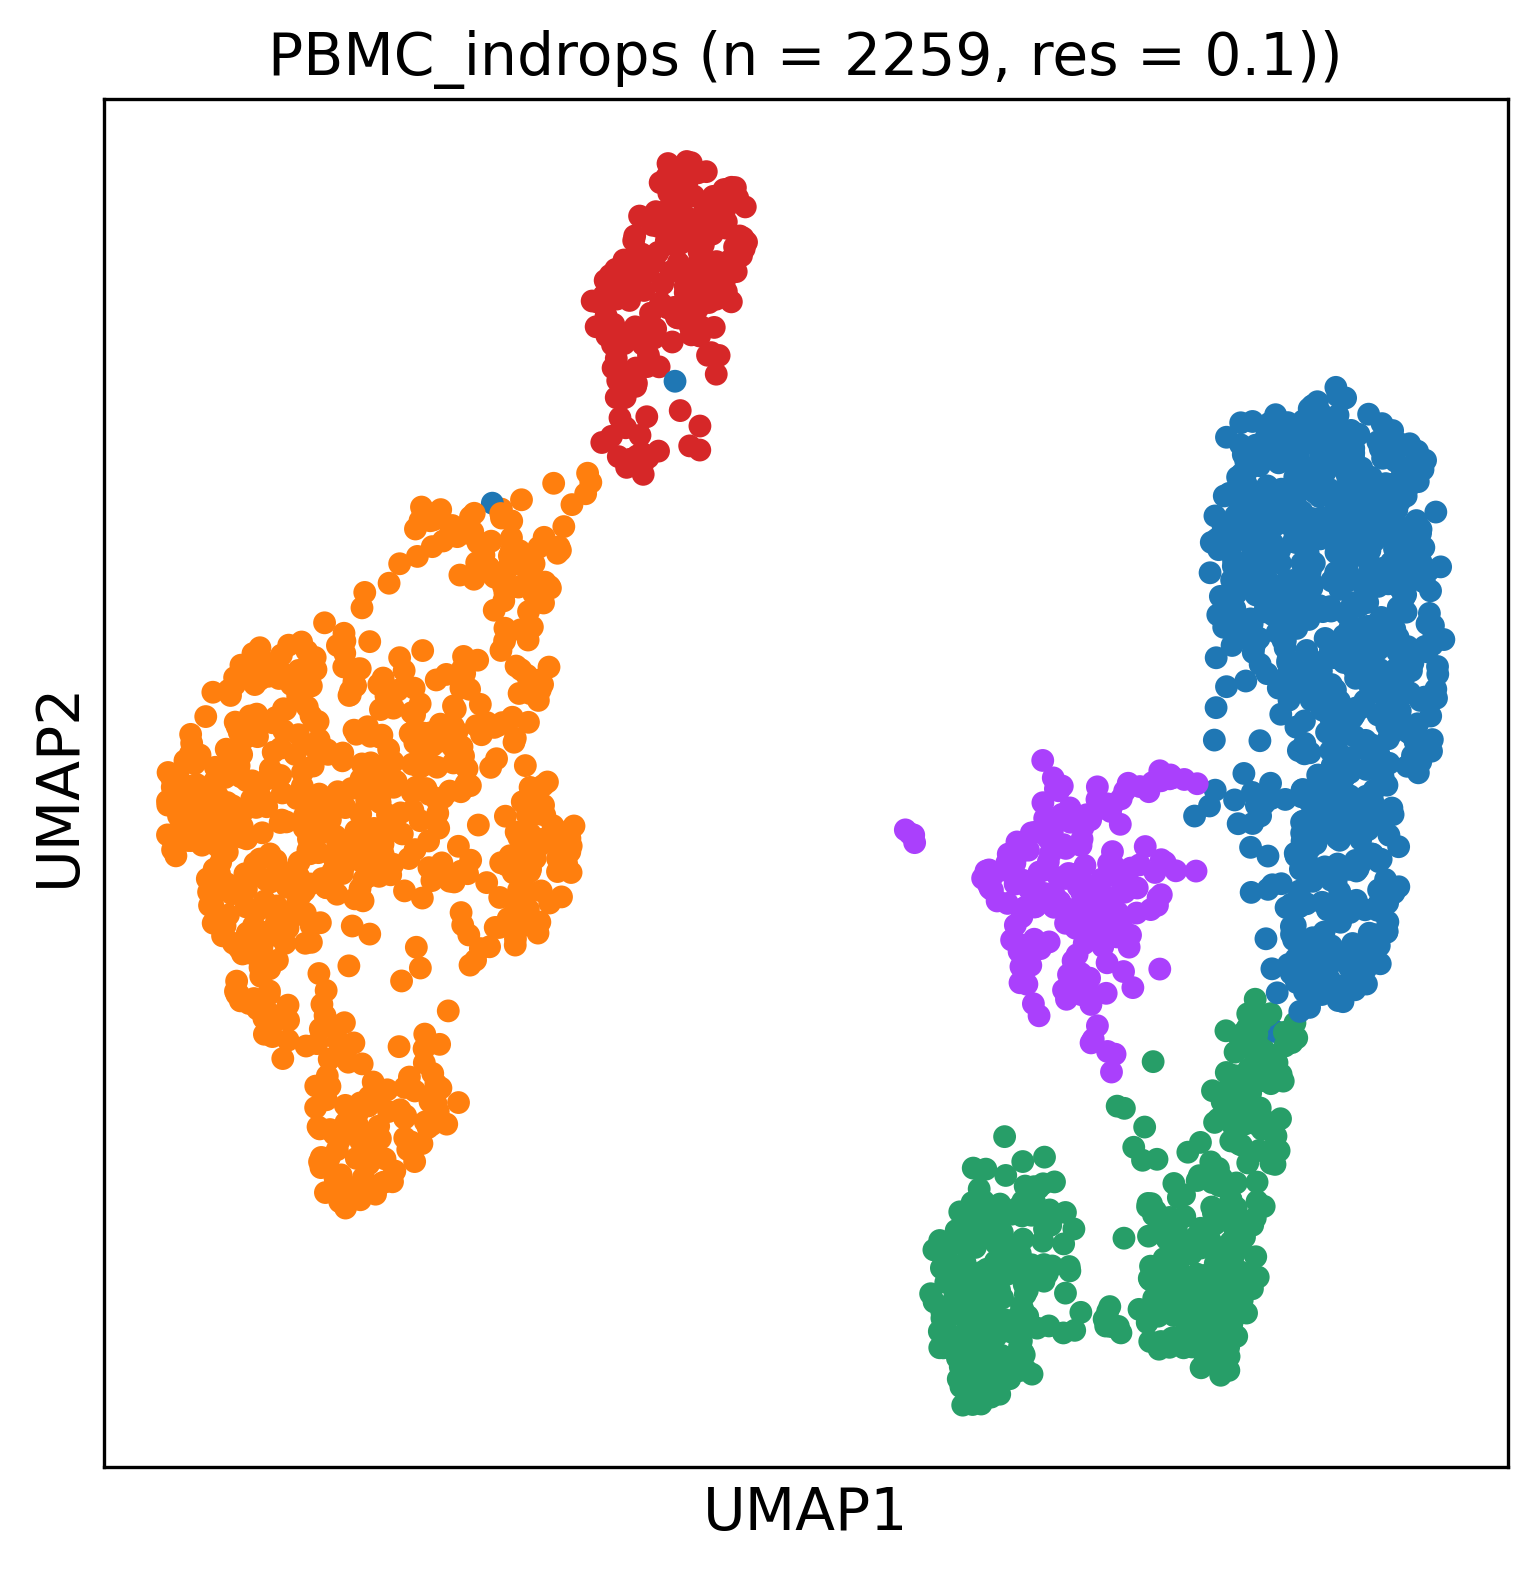
\includegraphics[width=0.25\textwidth]{images/clusterings/PBMC_indrops.png} &
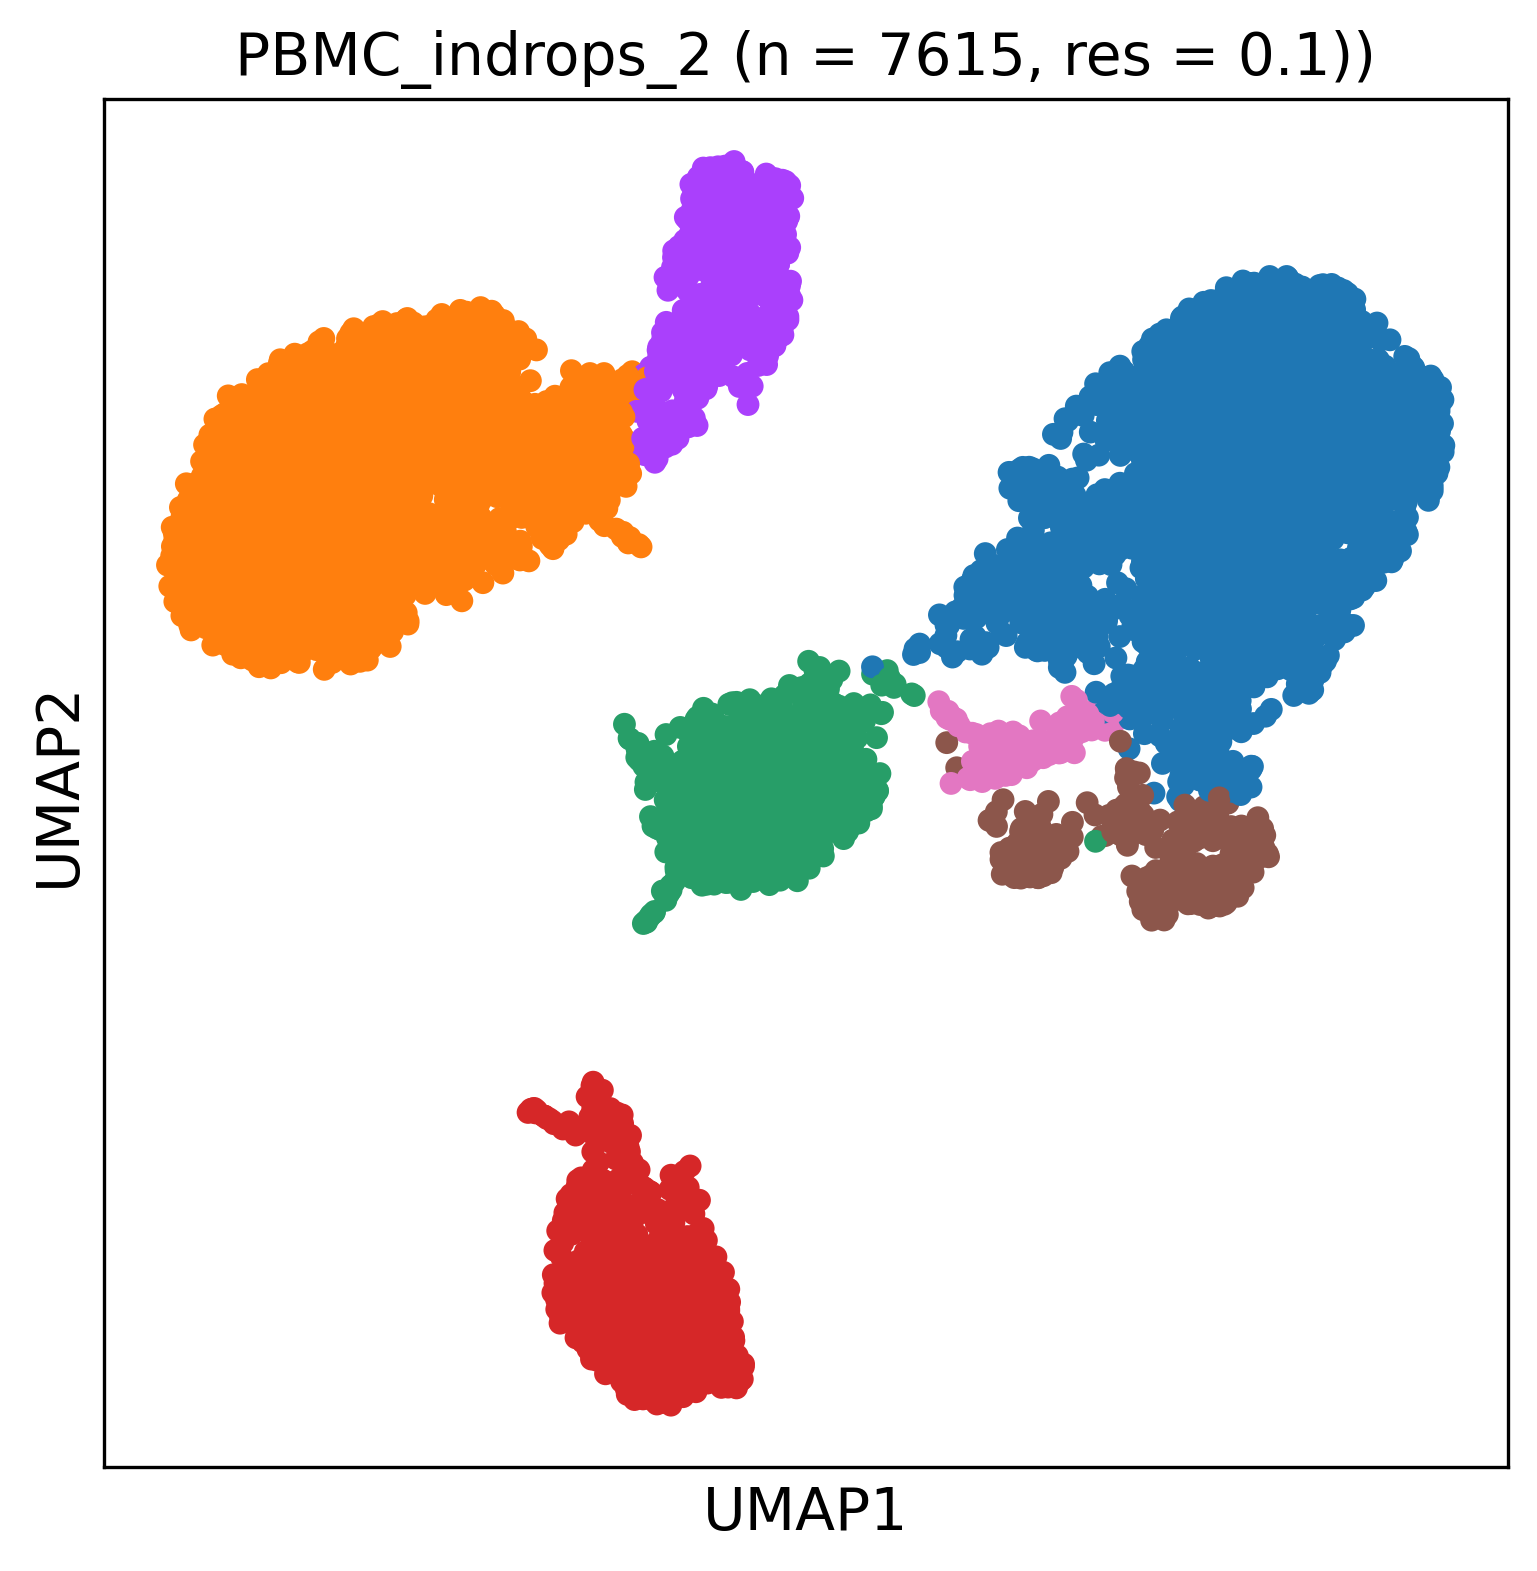
\includegraphics[width=0.25\textwidth]{images/clusterings/PBMC_indrops_2.png} &
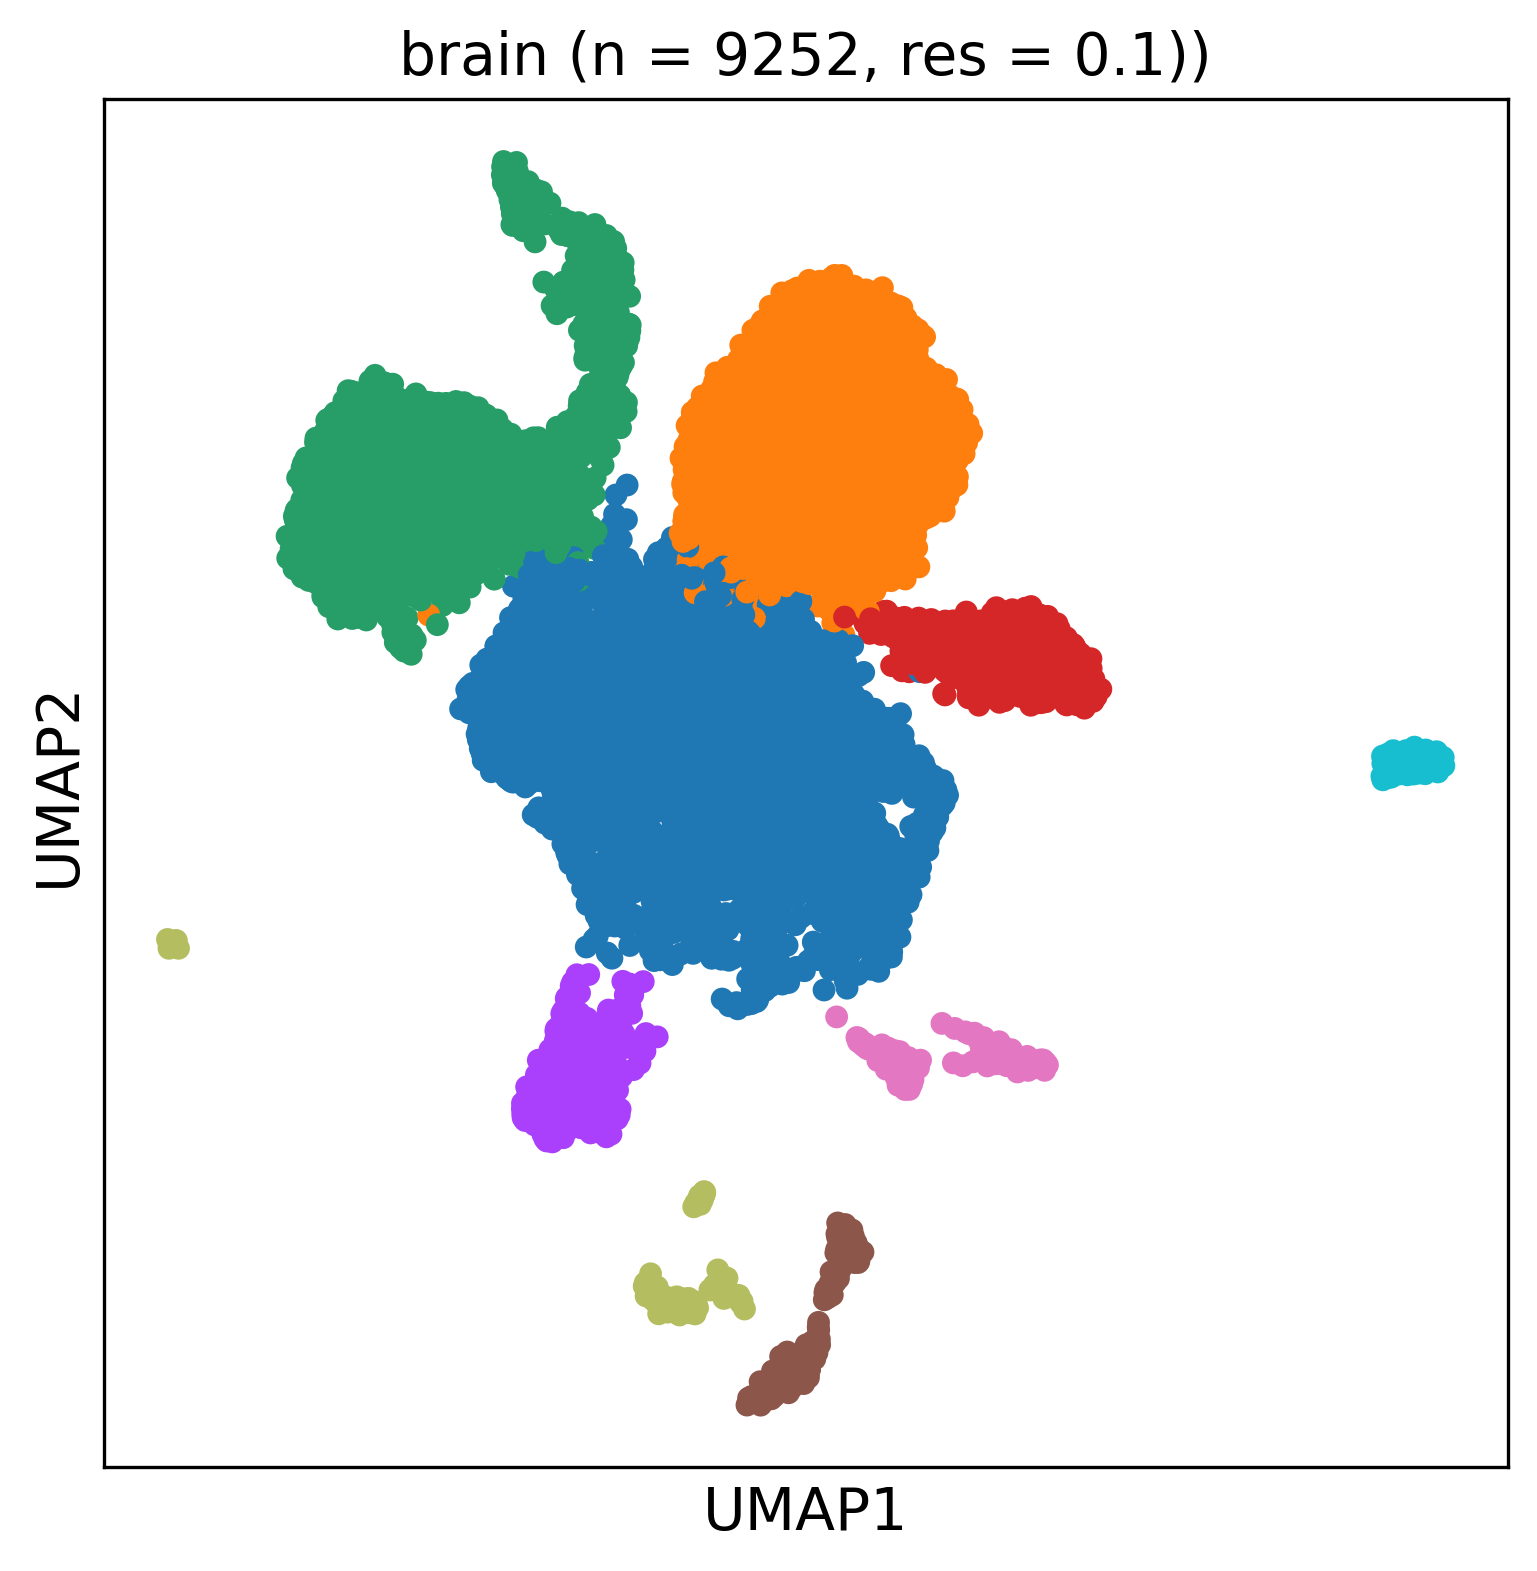
\includegraphics[width=0.25\textwidth]{images/clusterings/brain.png} \\
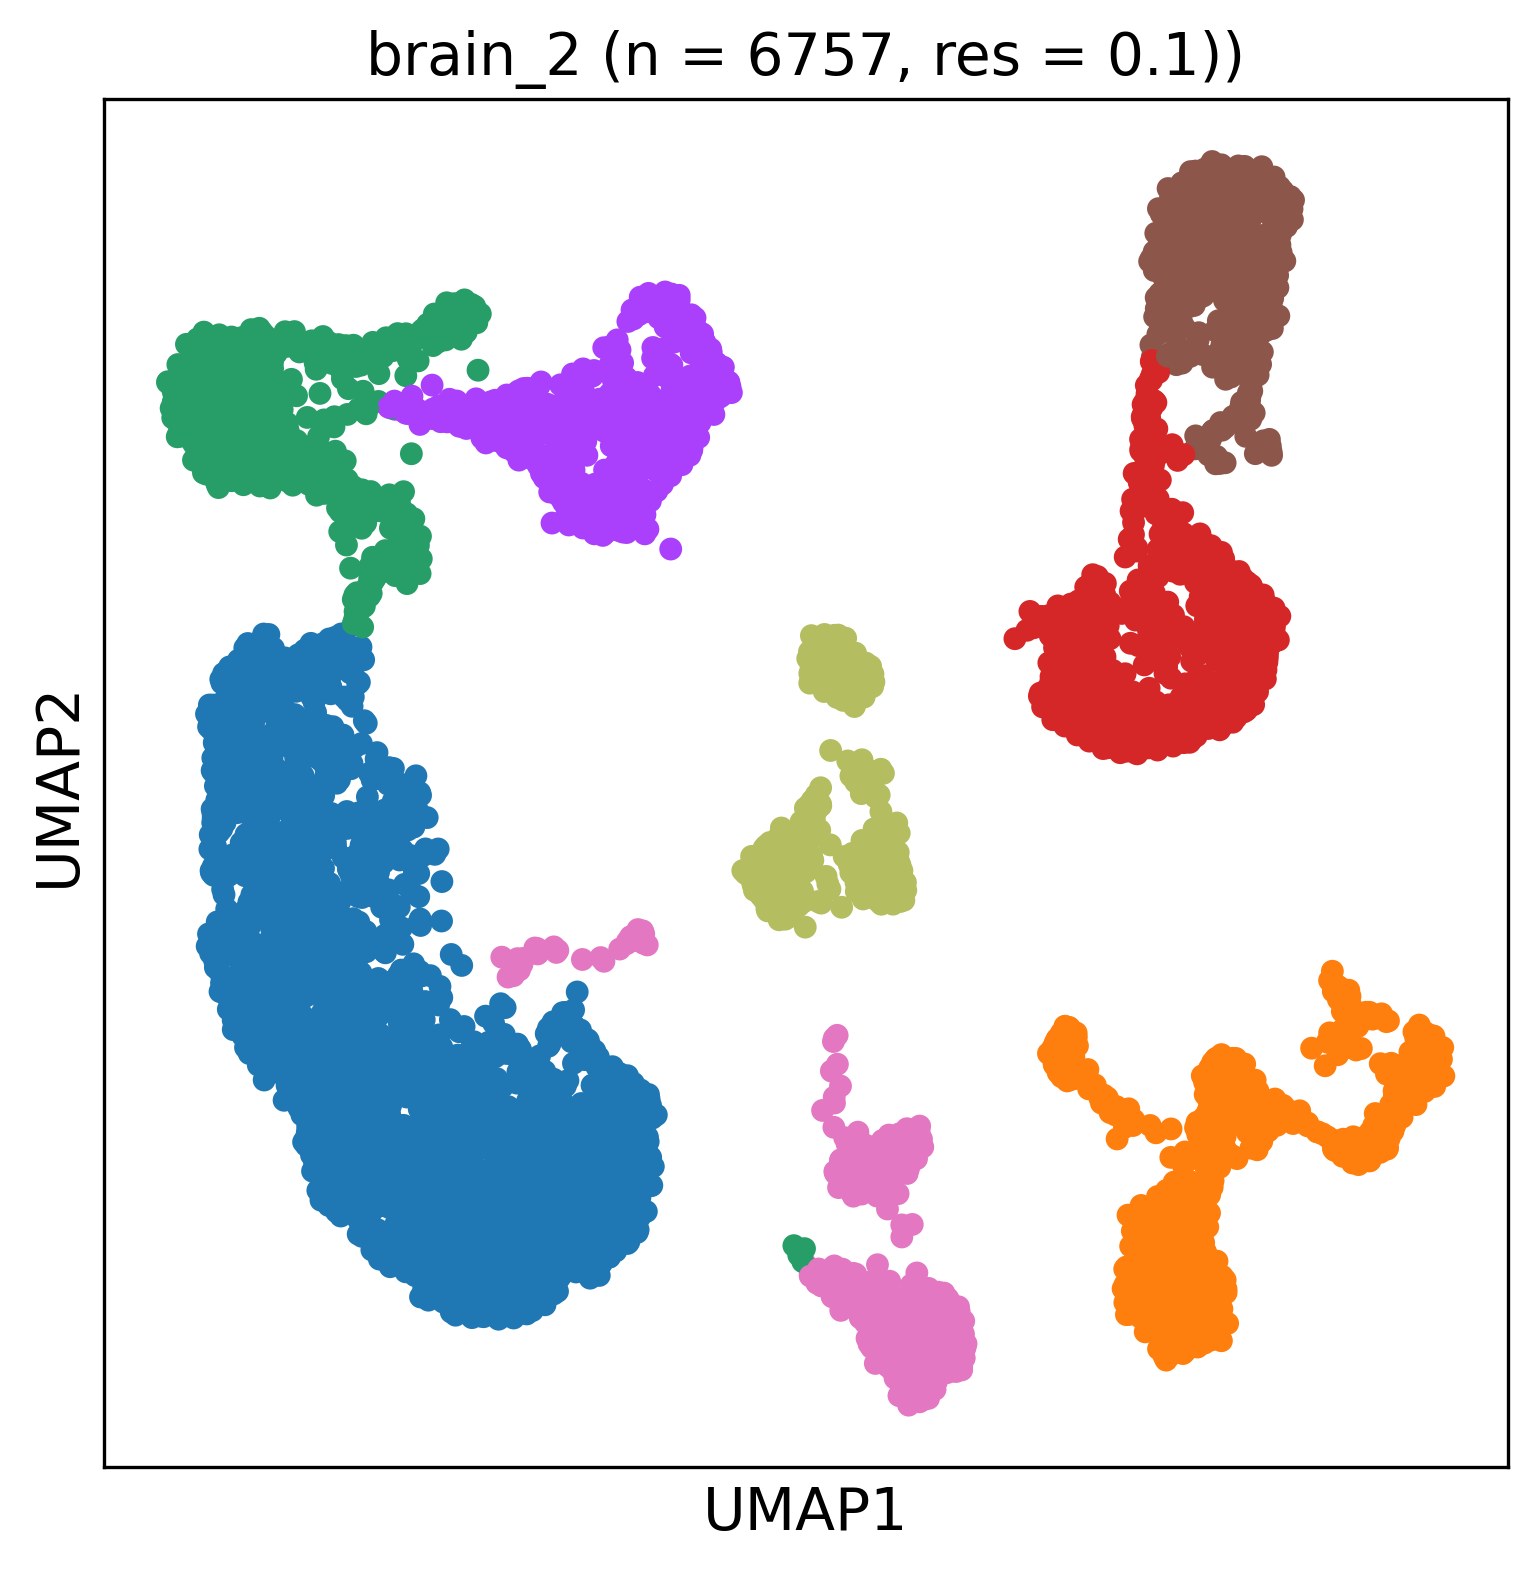
\includegraphics[width=0.25\textwidth]{images/clusterings/brain_2.png} &
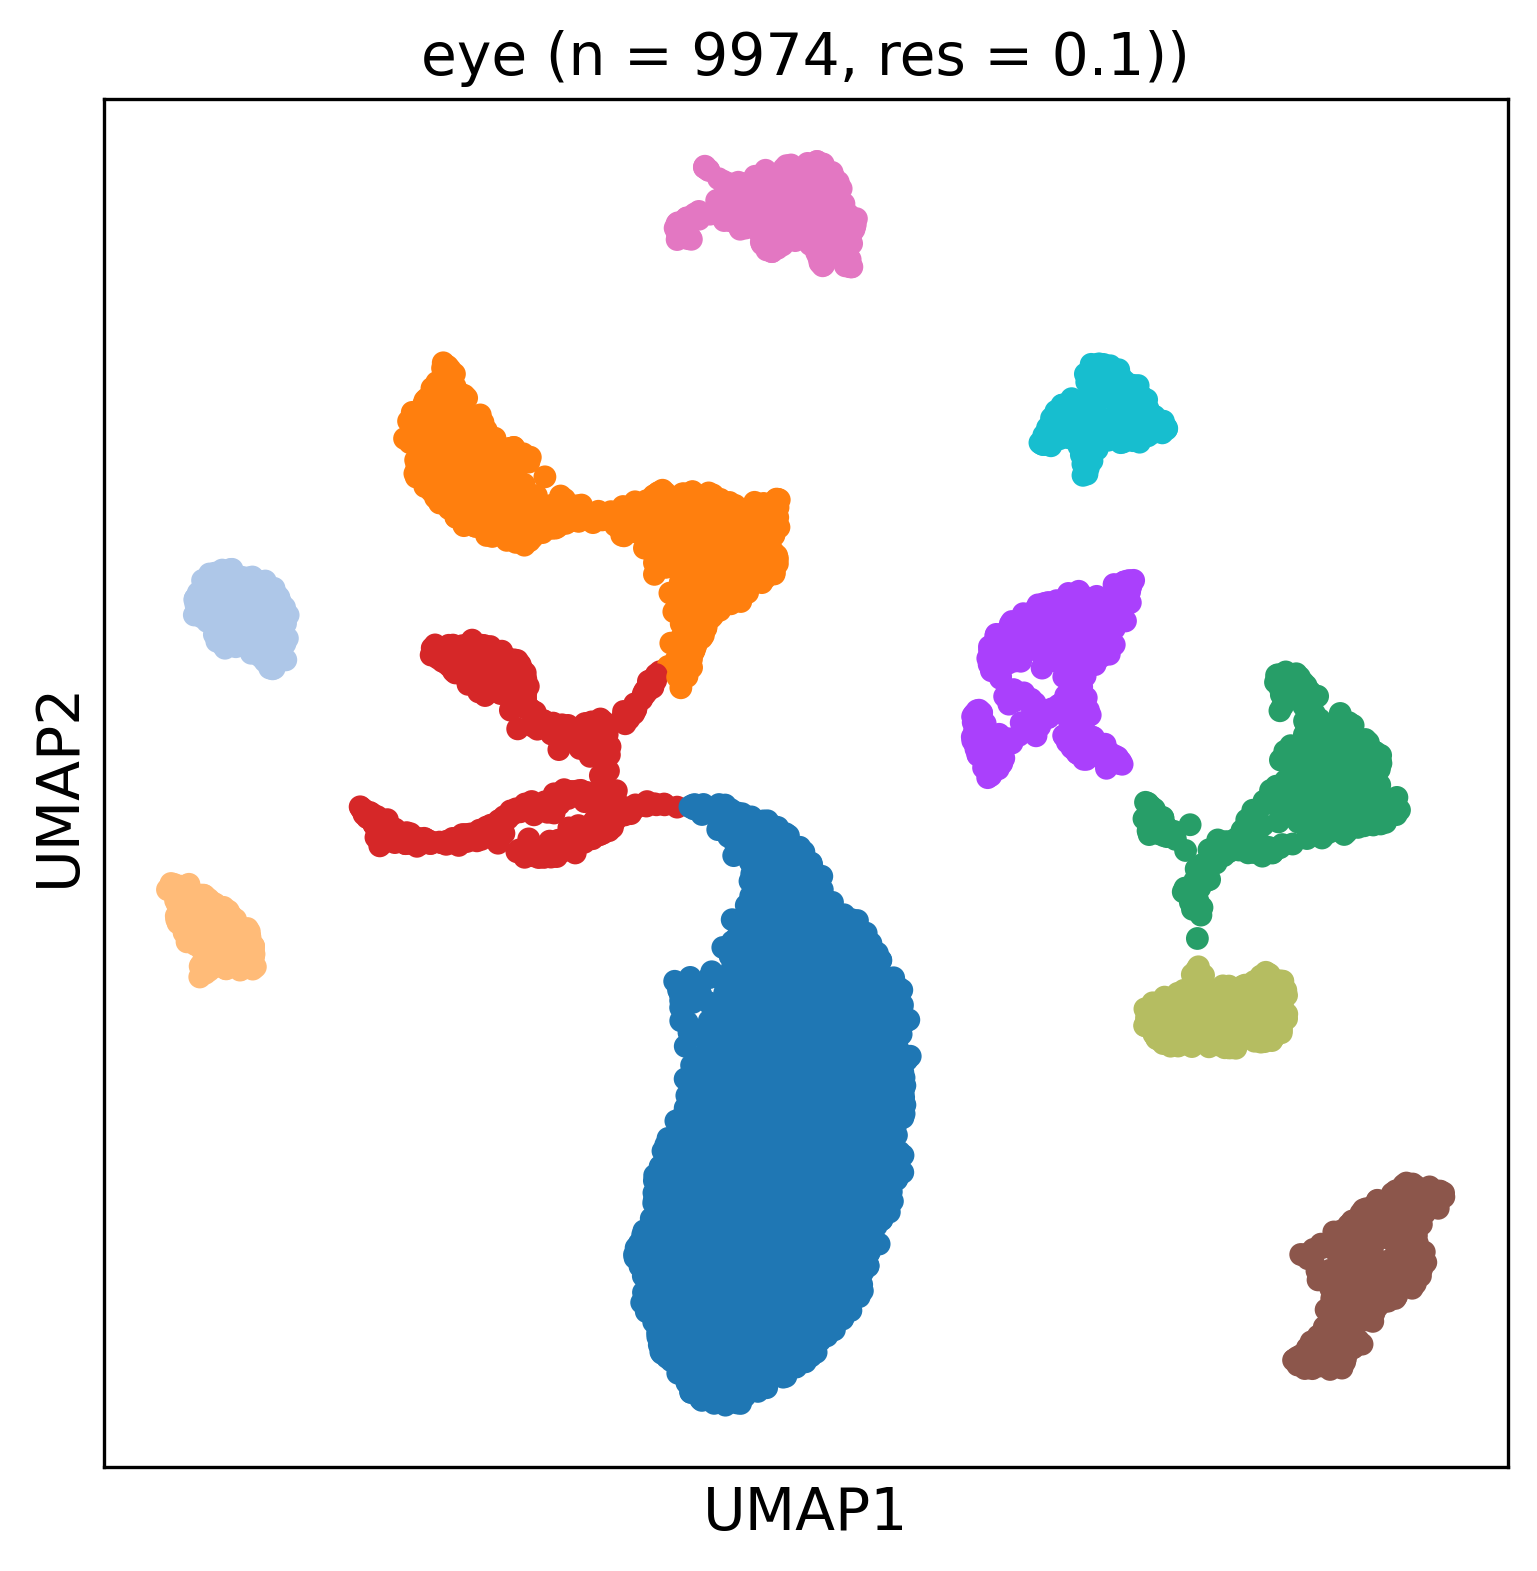
\includegraphics[width=0.25\textwidth]{images/clusterings/eye.png} &
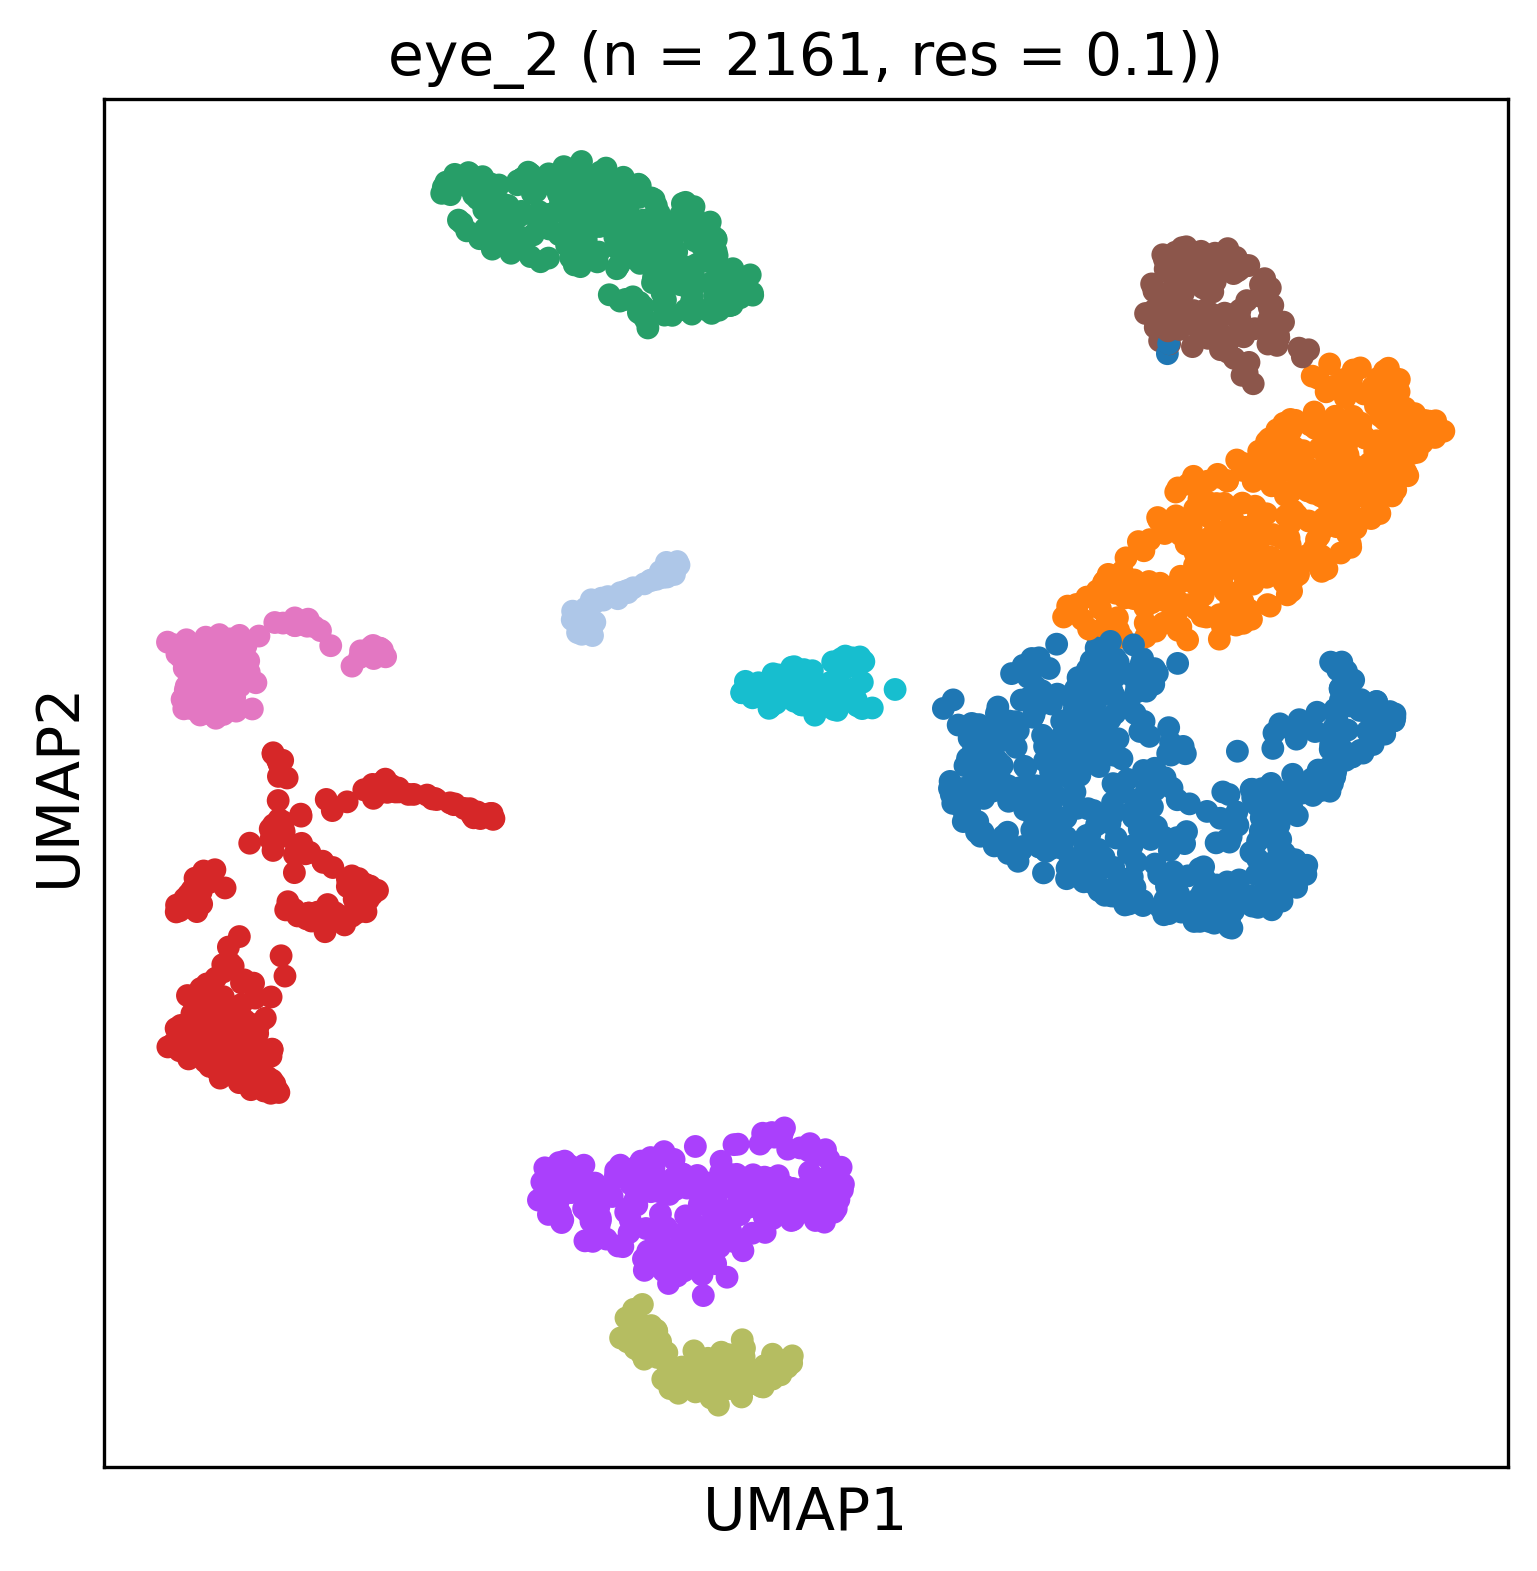
\includegraphics[width=0.25\textwidth]{images/clusterings/eye_2.png} \\
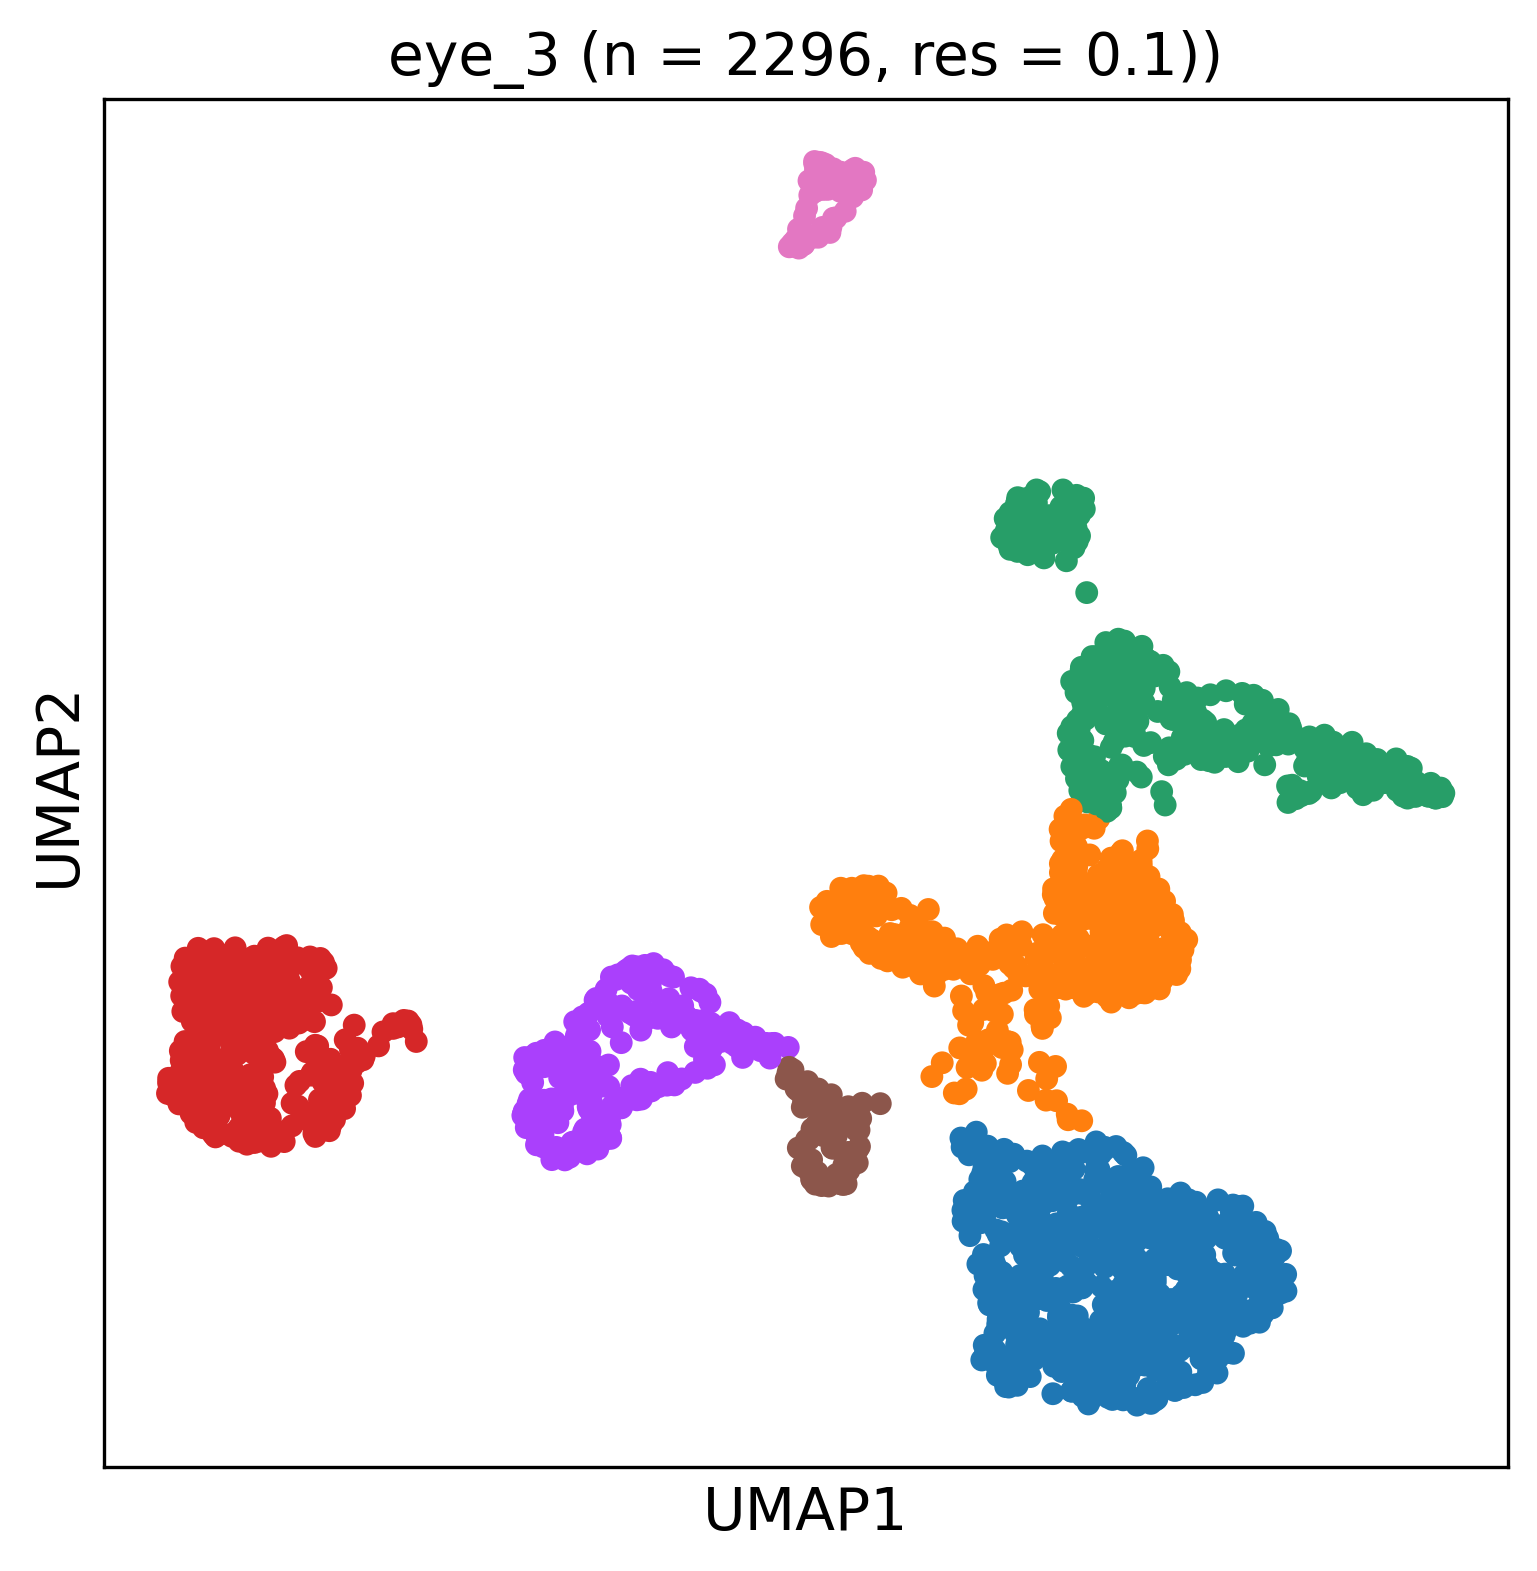
\includegraphics[width=0.25\textwidth]{images/clusterings/eye_3.png} &
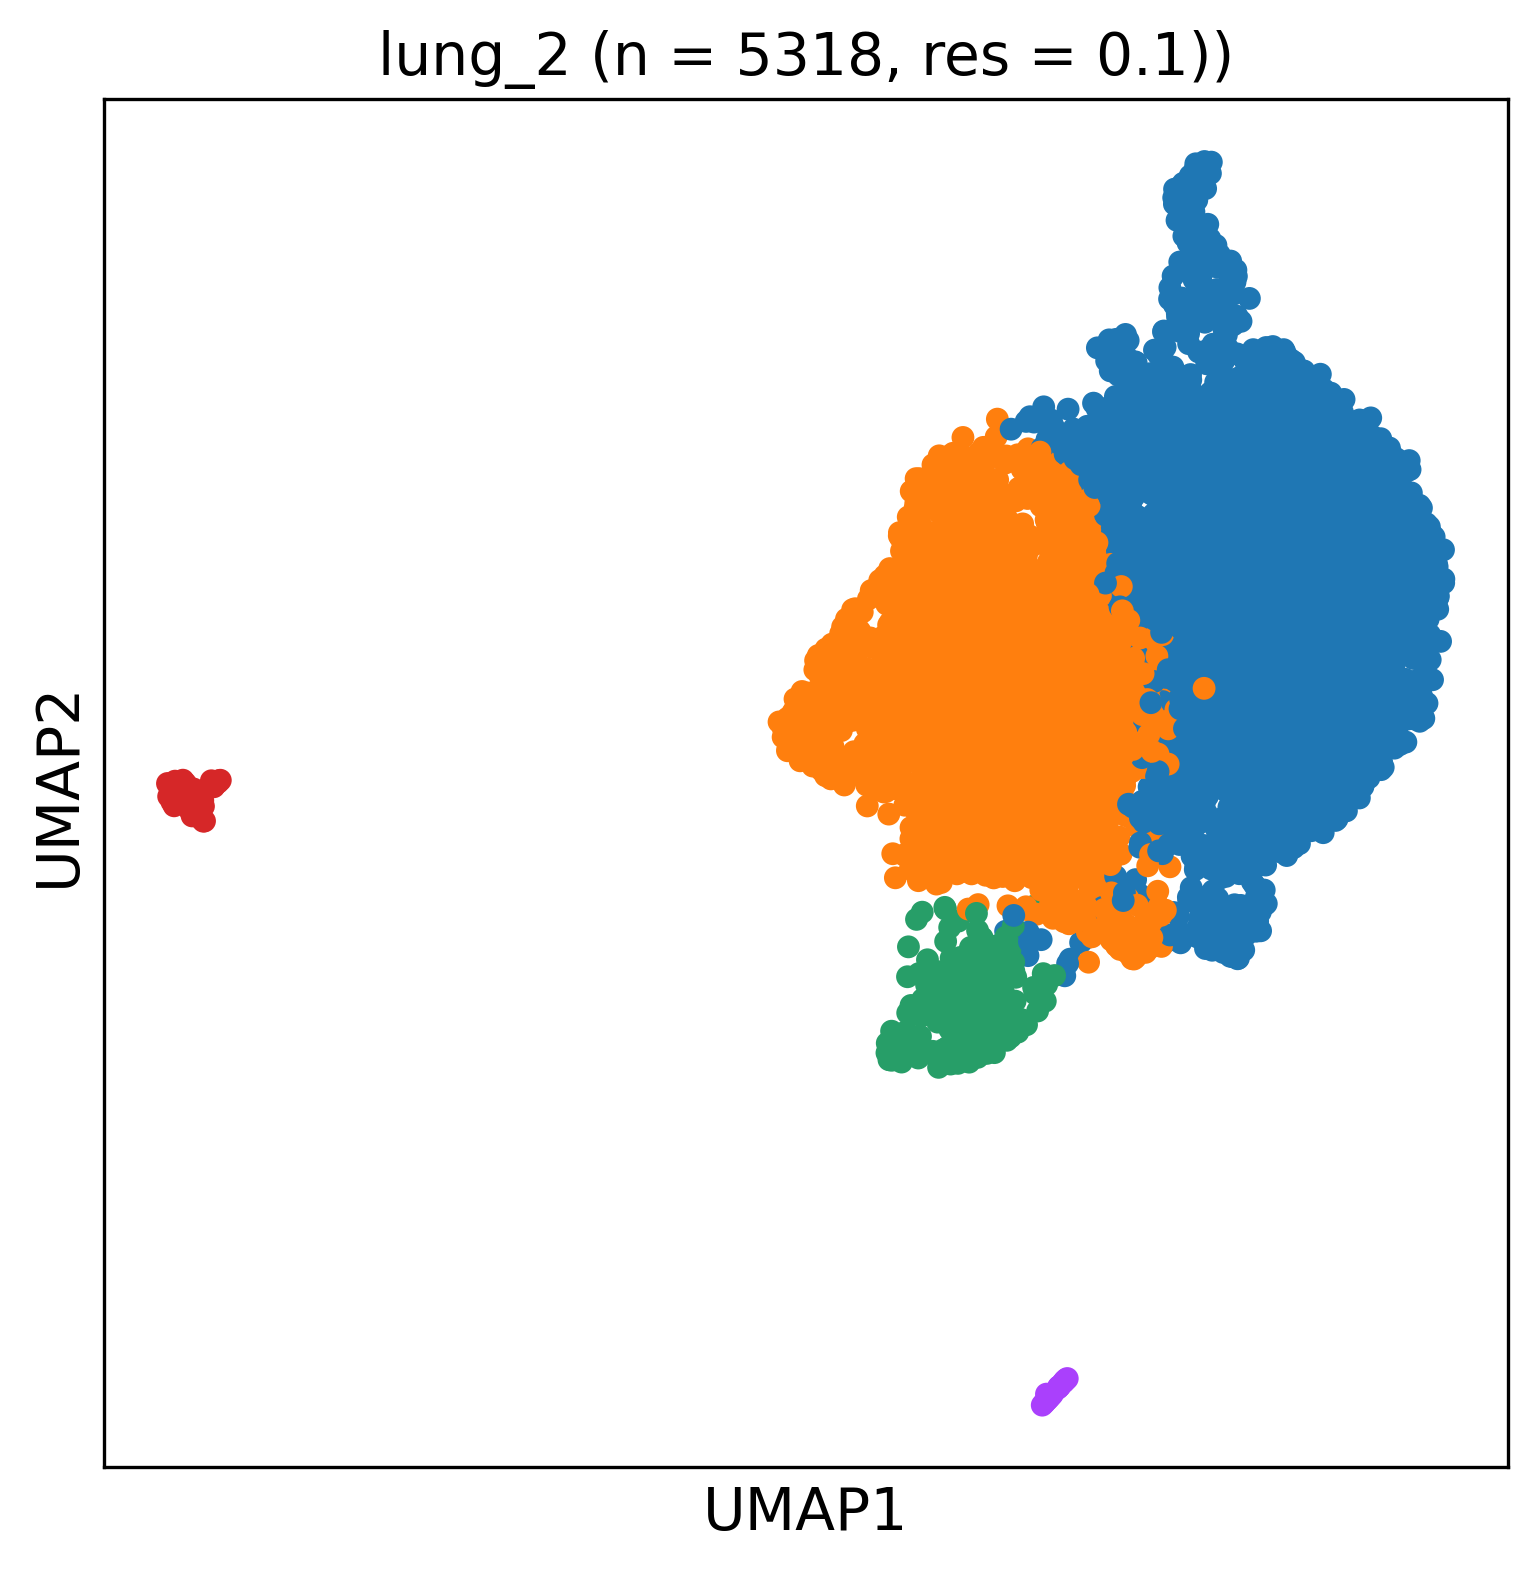
\includegraphics[width=0.25\textwidth]{images/clusterings/lung_2.png} &
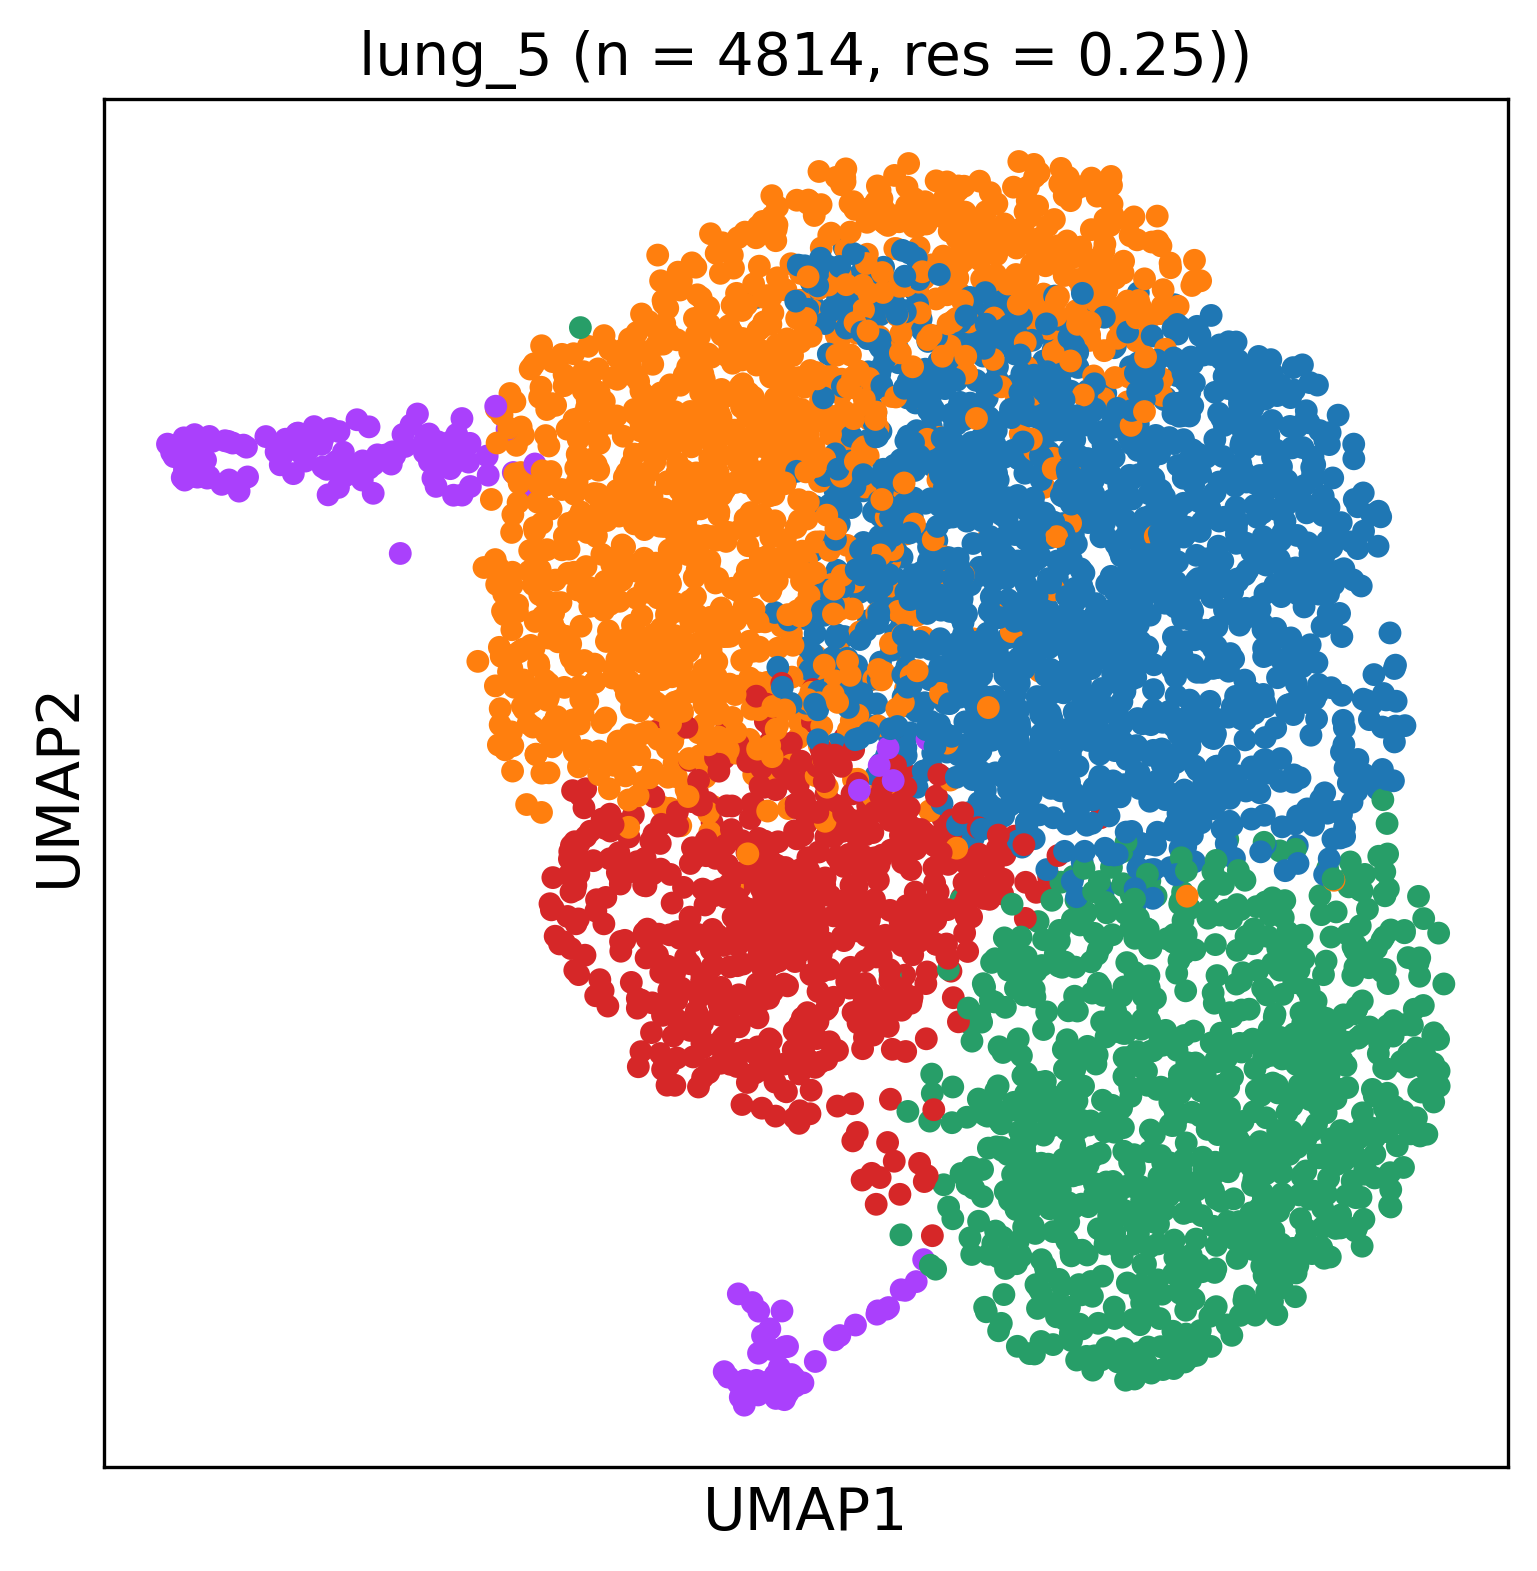
\includegraphics[width=0.25\textwidth]{images/clusterings/lung_5.png} \\
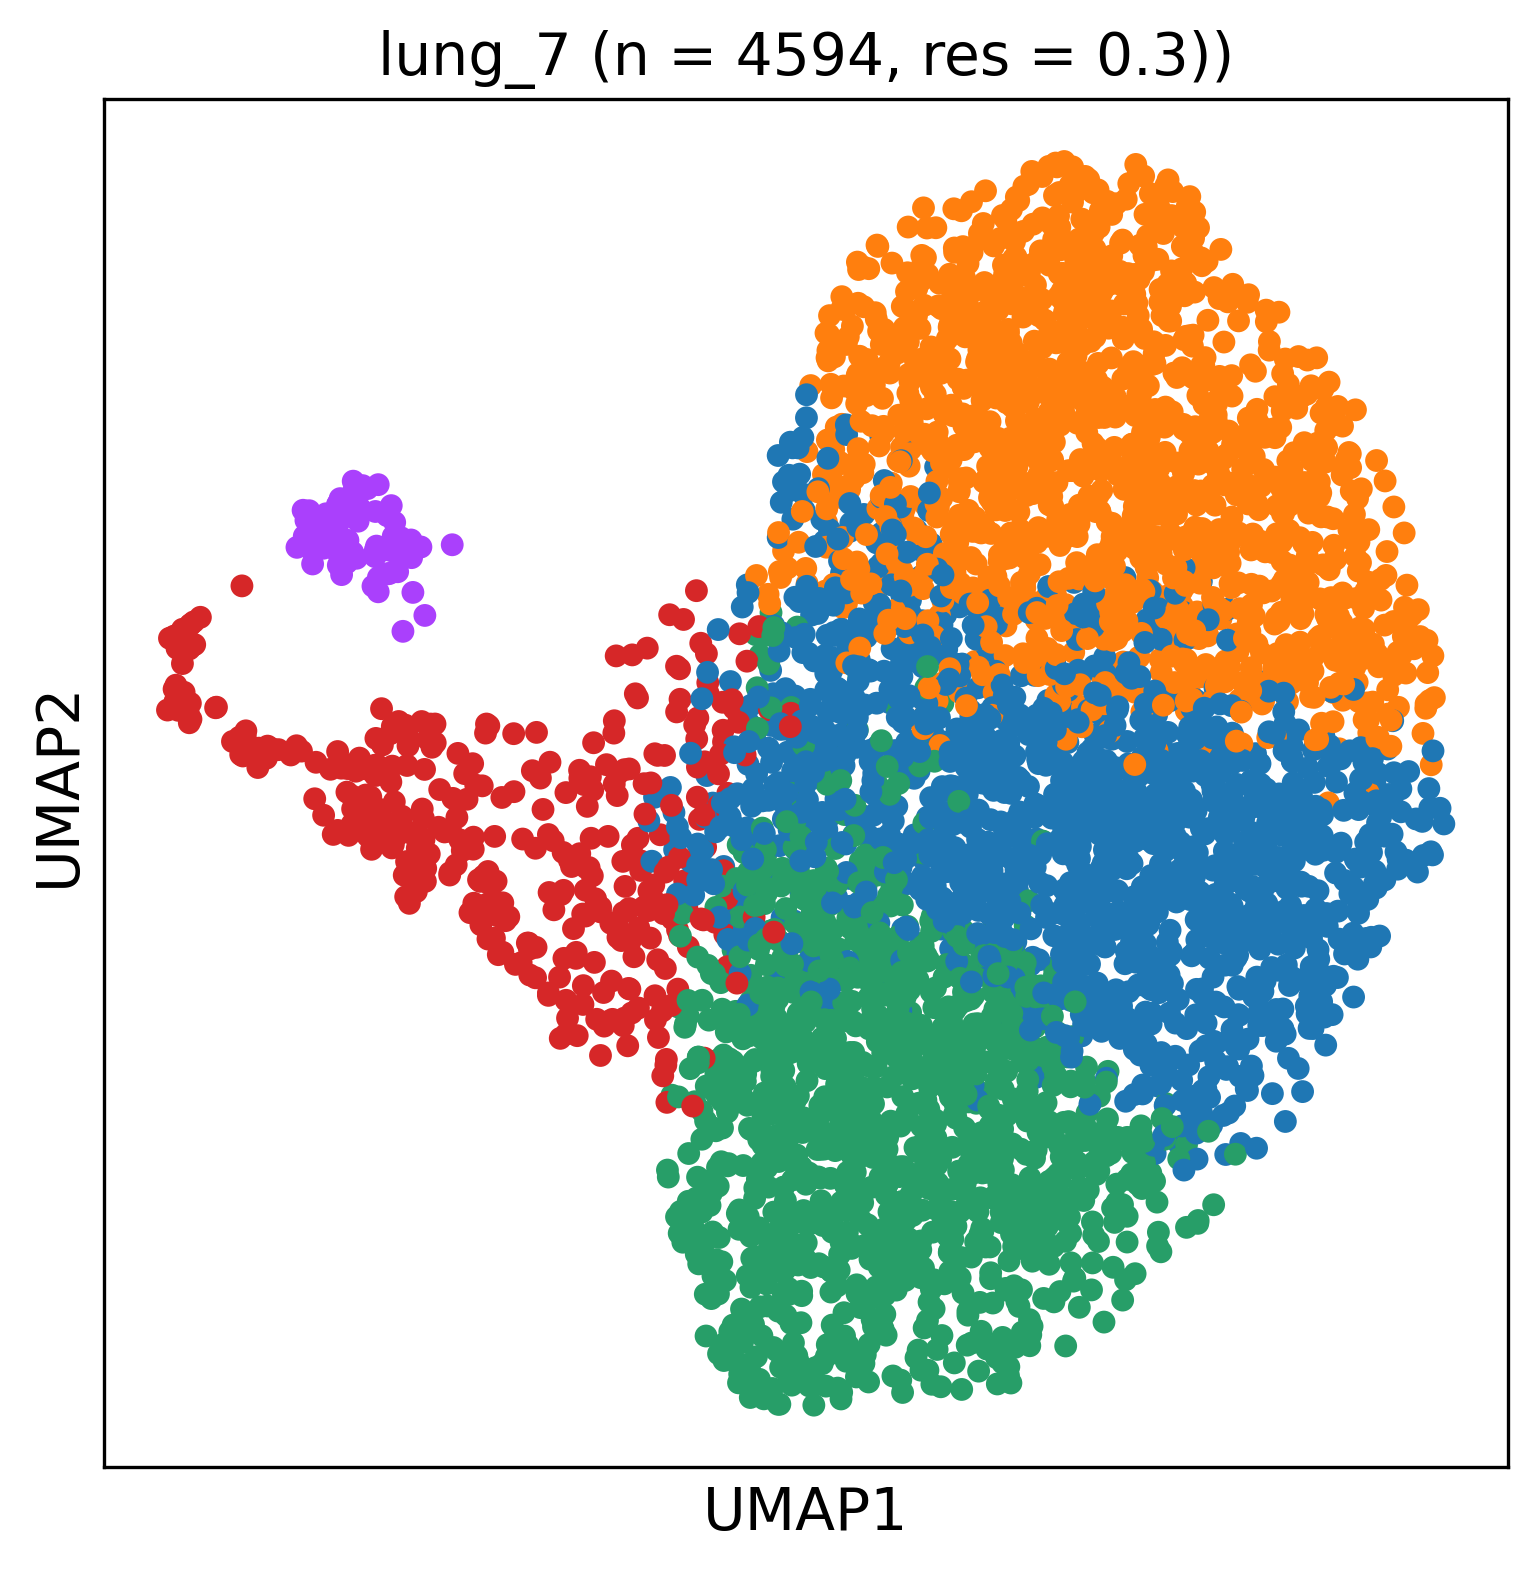
\includegraphics[width=0.25\textwidth]{images/clusterings/lung_7.png} &
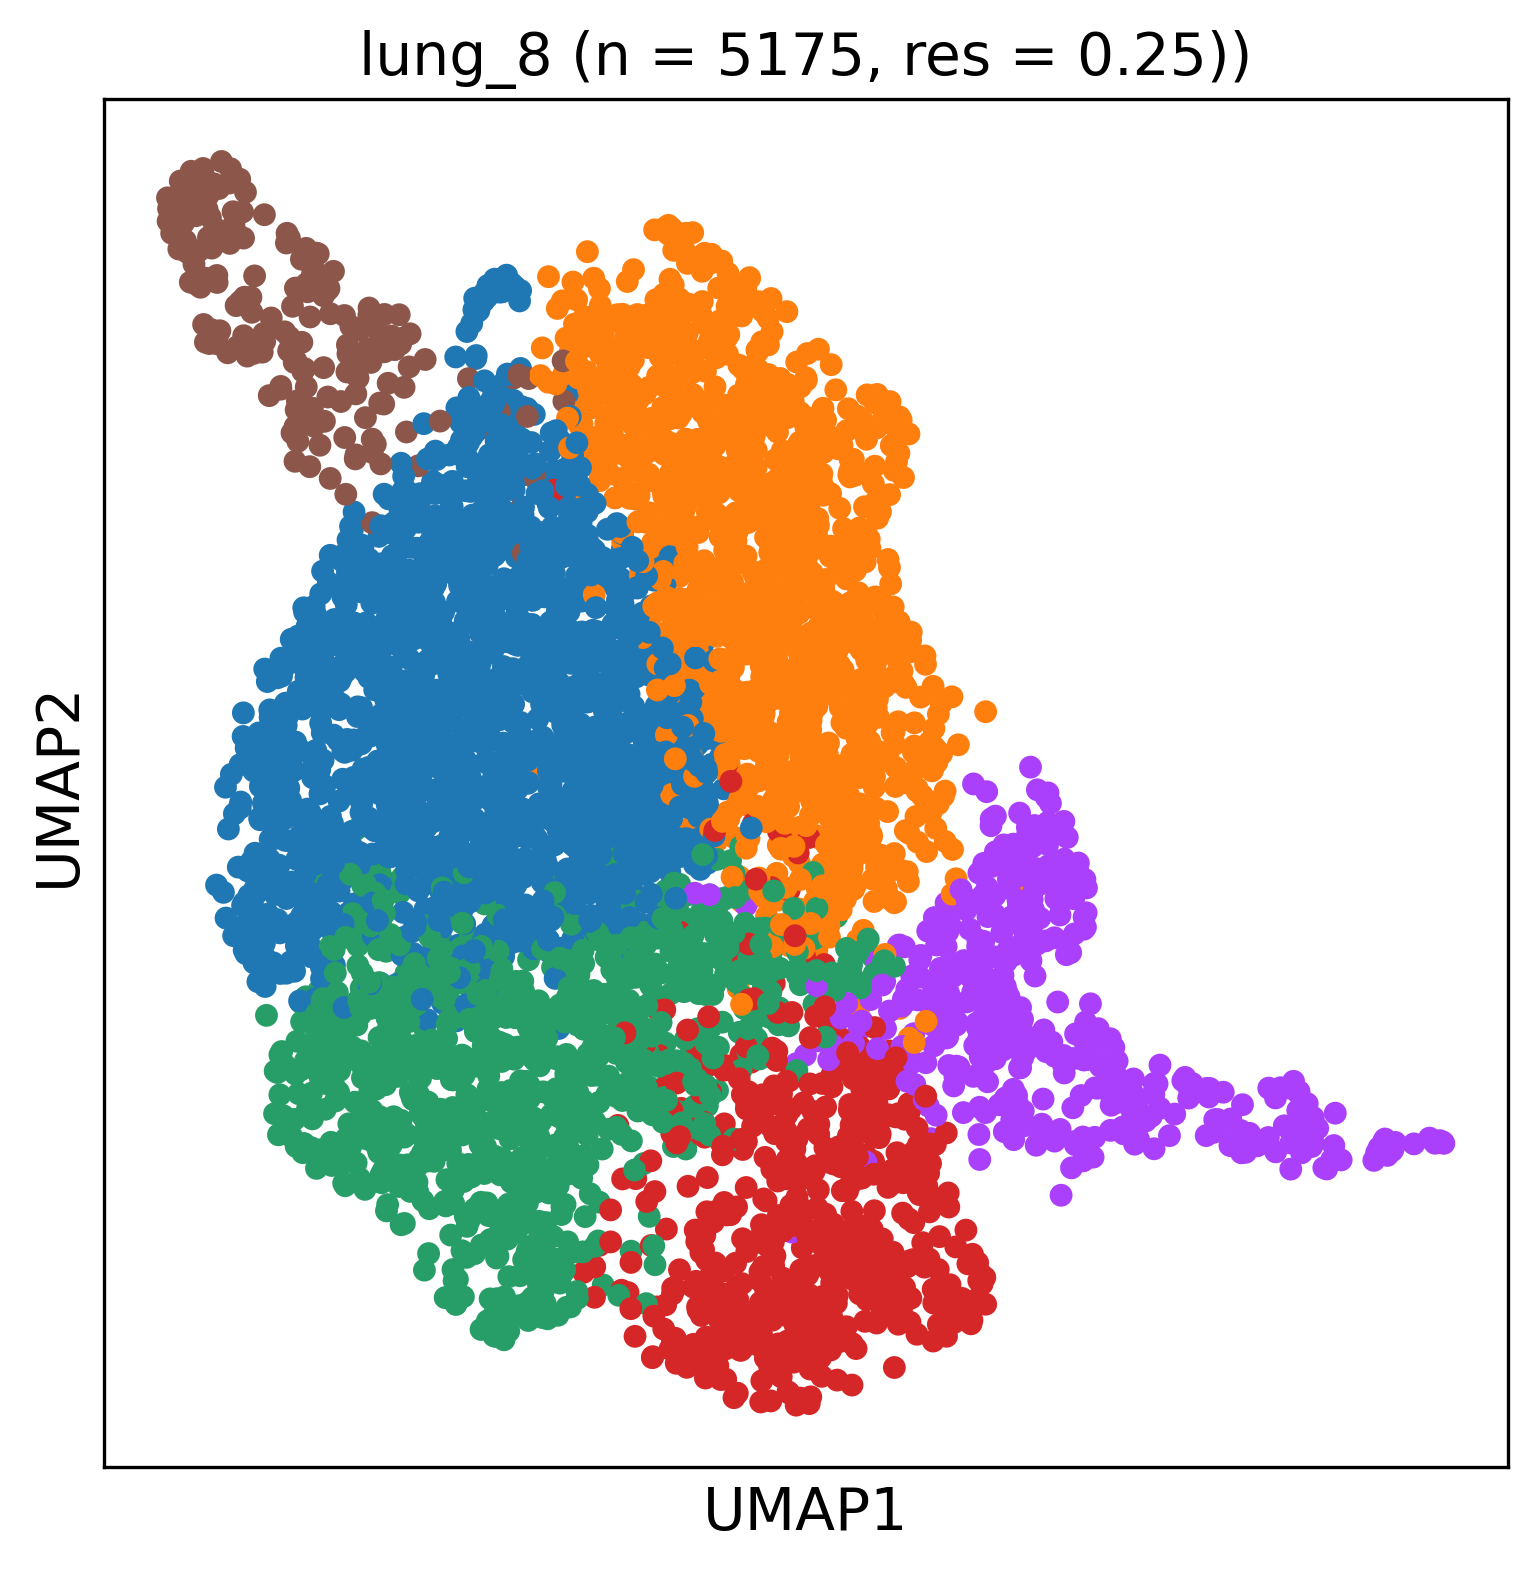
\includegraphics[width=0.25\textwidth]{images/clusterings/lung_8.png} &
\\
\end{tabular}
\caption{Clusterings of datasets. 'n' stands for number of cells in the plot, 'res' for the resolution parameter of leiden algorithm.
\textit{PBMC\_10x} samples are colored by CellTypist annotations.}
\label{fig:clusterings}
\end{figure}

\renewcommand{\arraystretch}{1.5}

\begin{longtable}{llccccc}
\caption{Isolated intergenic regions. The DGE column indicates whether the region is differentially expressed. The Predictions column shows whether the region overlaps with a predicted gene. The Conservation column indicates whether the region has a conservation score greater than 0.6. The TATA column shows the distance to the closest TATA box upstream (a dot indicates no TATA box was not found within 10 kb upstream). The Poly-A column shows the distance to the poly-A stretch downstream (negative values indicate cases where the poly-A stretch slightly overlaps with the defined region, dot indicate that such stretch was not found in the 1kb downstream).} 
\label{tab:isolated}\\
\toprule
Name & Coordinates & DGE & Predictions & Conservation & TATA & Poly-A \\
\midrule
\endfirsthead

\toprule
Name & Coordinates & DGE & Predictions & Conservation & TATA & Poly-A \\
\midrule
\endhead

\midrule
\multicolumn{7}{r}{\textit{Continued on next page}} \\
\bottomrule
\endfoot

\bottomrule
\endlastfoot

INT1066 & 16:11540750-11541200 & Yes & No & No & . & -10 \\
INT1312 & 3:141483900-141484100 & Yes & No & No & . & 25 \\
INT1366 & 12:14938950-14939300 & Yes & No & No & . & 33 \\
INT1426 & 12:10148500-10148700 & Yes & No & No & 307 & 21 \\
INT1483 & 16:11541550-11541700 & Yes & No & No & . & 74 \\
INT1492 & X:56386150-56386400 & Yes & No & No & 257 & 42 \\
INT1525 & 8:11842200-11842350 & Yes & Yes & No & . & 67 \\
INT1554 & 14:61119550-61119750 & Yes & No & No & . & 54 \\
INT1609 & 1:149879050-149879250 & Yes & No & No & . & 58 \\
INT1938 & 6:148107250-148107550 & Yes & No & No & . & 17 \\
INT196 & 6:89086200-89086500 & Yes & Yes & No & 713 & -2 \\
INT1993 & 6:43788000-43788200 & Yes & No & No & . & 45 \\
INT2008 & 17:1567900-1568100 & Yes & No & No & . & 22 \\
INT2141 & 6:159668300-159668550 & Yes & No & No & . & 37 \\
INT2209 & 9:93049900-93050150 & Yes & No & No & . & 21 \\
INT2328 & 1:991500-991800 & Yes & No & No & . & -44 \\
INT2456 & 13:113740250-113740500 & Yes & No & No & . & -10 \\
INT3259 & 17:35461800-35462050 & Yes & No & No & 150 & 22 \\
INT349 & 17:43322200-43322700 & Yes & No & No & . & 97 \\
INT368 & 19:14511650-14511900 & Yes & No & No & 231 & 42 \\
INT404 & 2:73747700-73748000 & Yes & No & No & 250 & 13 \\
INT4044 & 1:144412800-144413000 & Yes & No & No & . & . \\
INT4216 & 19:39430250-39430550 & Yes & No & No & . & 17 \\
INT4287 & 17:78646500-78646650 & Yes & No & No & . & 57 \\
INT4872 & 1:12153700-12153900 & Yes & No & No & . & 415 \\
INT5677 & 9:40875600-40875750 & Yes & No & No & . & 185 \\
INT5882 & 7:8754100-8754250 & Yes & No & No & 653 & 124 \\
INT6013 & 2:7102300-7102500 & Yes & No & No & . & 102 \\
INT977 & 1:145987350-145987600 & Yes & No & No & 879 & 37 \\
INT1002 & 5:82392950-82393200 & No & No & No & . & 71 \\
INT1020 & 2:218407950-218408200 & No & No & No & 881 & 59 \\
INT1114 & 21:15897200-15897400 & No & No & No & . & 42 \\
INT1173 & X:81313150-81313400 & No & No & No & 737 & 64 \\
INT1216 & 1:72282700-72282900 & No & Yes & Yes & . & -5 \\
INT127 & 17:32384850-32385100 & No & No & No & 656 & 51 \\
INT1385 & 2:86496700-86496900 & No & No & No & 89 & 12 \\
INT1387 & 11:63570800-63571050 & No & Yes & No & 231 & -26 \\
INT1406 & 14:21194850-21195150 & No & No & No & . & -50 \\
INT1428 & 3:88001700-88001900 & No & No & No & . & 47 \\
INT1467 & 5:112519400-112519600 & No & No & No & 765 & 6 \\
INT1470 & 17:32392900-32393100 & No & No & No & 670 & 118 \\
INT1509 & 2:42067000-42067200 & No & No & No & 95 & 27 \\
INT1527 & 19:7573150-7573300 & No & No & No & . & 38 \\
INT1542 & 18:70815200-70815400 & No & No & No & . & 22 \\
INT1549 & 1:231017800-231018000 & No & No & No & . & 48 \\
INT1569 & 1:157823400-157823600 & No & No & No & . & 11 \\
INT1571 & 10:17913700-17913900 & No & No & No & . & 21 \\
INT1579 & 3:12435200-12435400 & No & No & No & . & 30 \\
INT1618 & 8:16107400-16107550 & No & No & No & 228 & 40 \\
INT1619 & 3:56722050-56722300 & No & No & No & . & 1 \\
INT1637 & 4:81423000-81423200 & No & No & No & 702 & 40 \\
INT1640 & 17:7180650-7180850 & No & No & No & . & 33 \\
INT1675 & 11:65772750-65772950 & No & No & No & . & . \\
INT1716 & 9:27320000-27320200 & No & No & No & . & 49 \\
INT1778 & 2:222711150-222711300 & No & No & No & 96 & 67 \\
INT1779 & 3:189405250-189405400 & No & No & No & 141 & 61 \\
INT1781 & 20:50205450-50205650 & No & No & No & 72 & 36 \\
INT1801 & 5:151272550-151272700 & No & Yes & No & . & 43 \\
INT1817 & 1:42711550-42711800 & No & No & No & . & 29 \\
INT1829 & 1:77772950-77773050 & No & No & Yes & . & -30 \\
INT1869 & 13:30764850-30765000 & No & No & No & . & . \\
INT1970 & 2:55277900-55278150 & No & No & No & 421 & -4 \\
INT2044 & 19:4041150-4041400 & No & Yes & No & . & 22 \\
INT2071 & 15:84812500-84812800 & No & No & No & 773 & 39 \\
INT2080 & 2:218816950-218817250 & No & No & No & . & 111 \\
INT2088 & 8:19876500-19876650 & No & No & No & 699 & . \\
INT212 & X:44794800-44794950 & No & No & No & . & -43 \\
INT2142 & 12:54548650-54548850 & No & No & No & . & 63 \\
INT2162 & 17:16355850-16356050 & No & No & No & . & 46 \\
INT2199 & 6:148122550-148122750 & No & No & Yes & . & 74 \\
INT2208 & 5:18162950-18163100 & No & No & Yes & . & 93 \\
INT225 & 9:131570800-131571100 & No & No & No & 400 & -23 \\
INT2389 & 22:17731150-17731400 & No & No & No & 818 & 26 \\
INT2420 & 1:52681350-52681600 & No & No & No & 980 & 52 \\
INT2448 & 15:77040800-77041050 & No & No & No & . & 47 \\
INT2585 & 17:75300550-75300800 & No & No & No & 473 & 12 \\
INT2716 & 7:39812450-39812600 & No & No & No & . & 108 \\
INT2777 & 12:106347650-106347900 & No & No & No & . & 50 \\
INT2826 & 3:156825050-156825300 & No & No & No & 254 & 47 \\
INT2970 & 1:30727150-30727450 & No & No & No & . & 3 \\
INT312 & 9:127792200-127792400 & No & No & No & . & 57 \\
INT313 & 20:5540550-5540800 & No & No & No & . & 20 \\
INT316 & 2:157407250-157407500 & No & No & No & 237 & 42 \\
INT3329 & 12:124911350-124911600 & No & No & No & . & 19 \\
INT3330 & 10:26574800-26575050 & No & No & No & 107 & 39 \\
INT3432 & 11:2318900-2319500 & No & No & No & . & 32 \\
INT3472 & 1:234336450-234336650 & No & No & No & 516 & 80 \\
INT3506 & 2:94568900-94569100 & No & No & No & 601 & . \\
INT3519 & 5:166646400-166646600 & No & No & No & 273 & 121 \\
INT3521 & 1:234330500-234330750 & No & No & No & 767 & 97 \\
INT3543 & 13:83860250-83860700 & No & No & No & 836 & -25 \\
INT3636 & X:129412750-129413050 & No & No & Yes & . & 107 \\
INT3657 & 10:95078350-95078550 & No & No & No & 255 & 110 \\
INT3658 & 11:29999550-29999750 & No & No & No & 760 & 98 \\
INT3668 & 5:120107300-120107650 & No & No & No & . & -21 \\
INT3671 & 16:56859450-56859650 & No & No & No & . & 116 \\
INT3704 & 18:43159050-43159250 & No & No & No & 70 & 104 \\
INT3759 & X:129426200-129426450 & No & No & No & . & 108 \\
INT3940 & 4:157391550-157391750 & No & No & No & . & 96 \\
INT4032 & 3:15548800-15549000 & No & No & No & 843 & 121 \\
INT4047 & 21:33361700-33361900 & No & No & No & 143 & 39 \\
INT4070 & 4:47430500-47430700 & No & Yes & No & 934 & 90 \\
INT4147 & 1:34861500-34861700 & No & Yes & No & . & 609 \\
INT4174 & 7:128664300-128664550 & No & No & No & 439 & 39 \\
INT4224 & 8:43139250-43139600 & No & No & No & . & . \\
INT4225 & 6:110097900-110098100 & No & No & No & 115 & 95 \\
INT4236 & X:121756550-121756750 & No & No & No & . & 83 \\
INT426 & 14:24169950-24170200 & No & No & No & . & 29 \\
INT4328 & 17:45610750-45610900 & No & No & No & 835 & 80 \\
INT4364 & Y:20418250-20418500 & No & No & No & 241 & 49 \\
INT4394 & 19:40026900-40027100 & No & No & No & . & 89 \\
INT4401 & 9:101413900-101414100 & No & No & No & . & 47 \\
INT4454 & X:57773350-57773500 & No & No & No & 191 & 136 \\
INT4488 & 9:41567350-41567550 & No & No & No & 304 & -23 \\
INT4525 & 12:11599200-11599400 & No & No & No & 776 & 19 \\
INT4577 & 5:702050-702300 & No & Yes & No & 893 & 86 \\
INT4610 & 2:7218550-7218750 & No & No & No & 90 & 53 \\
INT4697 & 5:166509150-166509400 & No & No & No & 14 & 55 \\
INT4706 & 13:19811450-19811650 & No & No & No & 22 & 108 \\
INT480 & 17:32396150-32396400 & No & No & No & 137 & 26 \\
INT4851 & X:129410350-129410550 & No & No & No & . & 94 \\
INT4924 & 20:33358150-33358400 & No & No & No & . & 46 \\
INT4948 & 5:703250-703450 & No & Yes & No & . & . \\
INT4955 & 8:40521250-40521500 & No & No & No & 5 & 76 \\
INT4975 & 12:47660700-47660950 & No & No & No & 71 & . \\
INT5017 & 18:5389700-5389900 & No & No & No & . & 94 \\
INT5128 & 16:67010550-67010750 & No & No & No & . & 81 \\
INT5190 & 18:5386900-5387050 & No & No & No & . & 125 \\
INT5456 & 11:1269150-1269350 & No & No & No & . & 115 \\
INT5524 & 19:46024000-46024250 & No & No & No & 287 & 73 \\
INT560 & 6:32862450-32862700 & No & No & No & 102 & 34 \\
INT5710 & 4:47428500-47428700 & No & Yes & No & 594 & 91 \\
INT575 & 11:85955150-85955450 & No & No & No & . & -6 \\
INT5801 & 16:67010700-67010900 & No & No & No & 949 & . \\
INT5808 & 5:26875600-26875800 & No & No & No & 926 & 109 \\
INT584 & 2:171768300-171768600 & No & No & No & 768 & 13 \\
INT5848 & 16:3239750-3239950 & No & No & No & 488 & 35 \\
INT593 & 2:32331000-32331250 & No & No & No & 814 & 36 \\
INT600 & 22:47183900-47184150 & No & No & No & 22 & 59 \\
INT6019 & 3:49344550-49344850 & No & No & No & . & 57 \\
INT620 & 21:15883150-15883400 & No & No & No & . & 20 \\
INT801 & 15:44718950-44719200 & No & No & No & 386 & 10 \\
INT827 & 9:94111950-94112200 & No & Yes & No & 336 & 55 \\
INT896 & 2:98598550-98598850 & No & No & No & . & 11 \\
INT904 & 2:26138650-26138950 & No & No & No & . & 41 \\
INT906 & 14:92696800-92697050 & No & No & No & . & 18 \\
INT925 & 18:51087400-51087650 & No & No & No & 855 & 17 \\





\end{longtable}

